\chapter{THIẾT KẾ VÀ HIỆN THỰC HỆ THỐNG}

Thiết kế và hiện thực hệ thống là một phần không thể thiếu trong quá trình phát triển các hệ thống điều khiển và tự động hóa. Việc thiết kế và hiện thực hệ thống đảm bảo rằng hệ thống sẽ hoạt động đúng như các yêu cầu đặt ra. Do đó, việc thiết kế và hiện thực hệ thống là rất quan trọng trong quá trình phát triển và có vai trò quyết định đến sự thành công của dự án.

Trong phần tiếp theo sau đây sẽ trình bày về quy trình thiết kế và hiện thực hệ thống điều khiển một cánh tay robot thông qua giao thức OPCUA.
\section{Tổng quan hệ thống}

Ở phần tổng quan, nhóm sẽ đưa ra kiến trúc hệ thống mà nhóm sử dụng cho việc hiện thực ứng dụng điều khiển, đồng thời liệt kê một số thiết bị, công nghệ được ứng dụng trong đồ án này.

\subsection{Kiến trúc hệ thống}
Trong dự án này, nhóm sẽ vẫn giữ lại mô hình kiến trúc hệ thống đã đề xuất ở Đồ án chuyên nghành trước đó với kiến trúc gồm 3 module gồm: 
\begin{itemize}
    \item VR Application: App điều khiển cánh tay được phát triển trên thiết bị mới có tên là Oculus Quest 2, người dùng có thể điều khiển cánh tay trong môi trường thực tế ảo (Virtual Reality - VR) sẽ được giới thiệu ở phần tiếp theo. Trong môi trường VR người dùng sẽ tương tác với một mô hình 3D của cánh tay robot ( Digital-twin ), những thay đổi của mô hình 3D sẽ được ánh xạ sang cánh tay vật lý thông qua các tương tác điều khiển của người dùng. Trong môi trường VR cũng có 2 màn hình video được stream lên từ các camera tích hợp vào cánh tay thông qua OPC để người dùng có thể quan sát môi trường ngoài thực tế.
    \item Datacenter: Một module trung gian được tích hợp vào hệ thống với mục đích là thu thập thông tin từ các thiết bị, các server OPC. Datacenter tập trung, tổng hợp toàn bộ các thông tin thu thập được vào một OPC server duy nhất chạy trong Datacenter. Cơ chế hiện thực này giúp ta dễ dàng mở rộng hệ thống hơn: ta có thể nâng cấp, bổ sung thêm nhiều thiết bị để điều khiển, chạy OPC server trên các thiết bị đó và kết nối tới Datacenter. Datacenter lúc này sẽ trở thành một điểm tập trung của dữ liệu, mà người dùng chỉ cần truy cập vào thì có thể điều khiển mọi thiết bị, miễn là chúng đang kết nối tới Datacenter. Chưa hết, với sự tập trung dữ liệu như vậy, Datacenter còn có thể trở thành một gateway IoT và đưa dữ liệu lên Cloud cho những xử lý cao cấp hơn như học máy, phân tích dữ liệu lớn...
    \item Control: Module control bao gồm 1 Server OPC chạy trên máy tính nhúng Jetson Nano, và một cánh tay robot có tên Jetmax được tích hợp driver điều khiển và camera nhận diện kèm theo. Cánh tay vật lý này sẽ là mô hình ánh xạ của cánh tay 3D trong môi trường VR, bất cứ tương tác nào trong VR cũng sẽ được cánh tay vật lý thực hiện theo. Người dùng có thể điều khiển cánh tay Jetmax thông qua 2 thiết bị khác nhau gồm VR Application trên Oculus Quest 2 với nhiều tính năng nổi bật như các dịch vụ AI và video streaming hoặc có thể điều khiển những chuyển động xoay cơ bản của cánh tay thông qua thiết bị cầm tay có tên là Joystick.
\end{itemize}

Dưới đây là sơ đồ kiến trúc của hệ thống:
\begin{figure}[!h]
    \centering
    \includegraphics[width=1\textwidth]{Images/architect_1.jpg}
    \caption{Kiến trúc hệ thống}
    \label{fig:comp_mqtt}
\end{figure}

Link github của dự án có thể được tìm thấy ở đây: \href{https://github.com/trong2409/Do_an_KTMT/tree/master}{https://github.com/trong2409\\/Do\_an\_KTMT/tree/master}

\subsection{Giới thiệu thiết bị và công nghệ}
Để thực hiện đồ án này, nhóm đã sử dụng kính thực tế ảo Oculus Quest 2 để phát triển ứng dụng VR trên Unity3D cho người dùng tương tác với cánh tay, một máy tính nhúng Rasberry Pi để chạy Datacenter, một máy tính nhúng khác có tên là Jetson Nano để chạy Server OPC và điều khiển cánh tay Jetmax thông qua các dòng lệnh ROS ( Robot Operating System ) đã được tích hợp sẵn vào Jetson Nano. Phần tiếp theo dưới đây sẽ trình bày rõ hơn về các thiết bị cũng như công nghệ được sử dụng trong đề tài.
\subsubsection{Oculus Quest 2}
Oculus Quest 2 là một thiết bị thực tế ảo (VR) độc lập, có thể được sử dụng mà không cần kết nối với một máy tính hoặc điện thoại thông minh. Nó được phát triển bởi công ty Oculus, một công ty con của Facebook, và ra mắt vào năm 2020.

Oculus Quest 2 được trang bị hai màn hình OLED độ phân giải 1832 x 1920 pixel trên mỗi mắt, cung cấp hình ảnh sắc nét và màu sắc chân thực. Nó cũng được trang bị bộ xử lý Snapdragon XR2, cung cấp hiệu suất mạnh mẽ để chạy các trò chơi và ứng dụng VR.

Với khả năng theo dõi chuyển động 6 độ tự do, Oculus Quest 2 cho phép người dùng di chuyển tự do trong không gian thực tế ảo, tạo ra trải nghiệm tuyệt vời cho người dùng. Nó cũng đi kèm với hai bộ điều khiển Oculus Touch để kiểm soát và tương tác với thế giới ảo.

Trong đồ án này, Oculus Quest 2 được sử dụng trong vài trò là 1 client cho người dùng tương tác với mô hình 3D của cánh tay được xậy dưng trong Unity, người dùng có thể điều khiển và sử dụng các tính năng AI được phát triển trên Jetmax thông qua Oculus.
\begin{figure}[!h]
    \centering
    \includegraphics[width=0.6\textwidth]{Images/Implementation/VRapp/Oculus.jpg}
    \caption{Hình ảnh Oculus Quest 2}
    \label{fig:comp_mqtt}
\end{figure}
\subsubsection{Rasberry Pi}
Raspberry Pi là một máy tính nhỏ gọn, có kích thước không lớn hơn một thẻ tín dụng. Nó được phát triển tại Vương Quốc Anh bởi Raspberry Pi Foundation với mục đích khuyến khích việc học lập trình và phát triển các ứng dụng thông qua các dự án sáng tạo.

Raspberry Pi có thể được sử dụng để thực hiện một loạt các tác vụ, bao gồm xây dựng các hệ thống điều khiển, phát triển phần mềm, thiết kế và xây dựng các thiết bị Internet of Things (IoT), học máy và trí tuệ nhân tạo, và nhiều ứng dụng khác.

Máy tính này được trang bị một bộ vi xử lý ARM, bộ nhớ RAM, các cổng kết nối USB, cổng Ethernet, cổng HDMI, và khe cắm thẻ nhớ microSD để lưu trữ dữ liệu. Nó cũng có thể được kết nối với các phụ kiện khác như camera, màn hình cảm ứng, micro, và các thiết bị điều khiển.

Với chi phí thấp, tính linh hoạt và dễ sử dụng, Raspberry Pi đã trở thành một lựa chọn phổ biến cho các nhà phát triển, giáo viên và sinh viên, người hâm mộ công nghệ và các tín đồ DIY (làm đồ tự chế). Raspberry Pi cũng được sử dụng rộng rãi trong giáo dục và các dự án nghiên cứu khác.

Trong đồ án này, máy tính nhúng Rasberry Pi được sử dụng để chạy module trung gian Datacenter, là nơi thu thập và chuyển tiếp dữ liệu cho 2 module VR Application và Control
\begin{figure}[!h]
    \centering
    \includegraphics[width=0.6\textwidth]{Images/Implementation/Datacenter/Ras.jpg}
    \caption{Hình ảnh của Rasberry Pi}
\end{figure}
\subsubsection{Jetson Nano và Jetmax Arm}
Jetson Nano là một bo mạch phát triển dành cho trí tuệ nhân tạo (AI) và học sâu (Deep Learning), được phát triển bởi NVIDIA. Với kích thước nhỏ gọn, Jetson Nano được trang bị một bộ vi xử lý ARM Cortex-A57 64 bit và một đồng xử lý đồ hoạ NVIDIA Maxwell GPU với 128 nhân CUDA.

Jetson Nano cũng có khả năng xử lý hình ảnh và video với tốc độ cao, cho phép nó được sử dụng để phát triển các ứng dụng nhận dạng hình ảnh, phân loại, giám sát và điều khiển trong các lĩnh vực như xe tự lái, robot, y tế và an ninh.

Bo mạch phát triển này cũng được trang bị các cổng kết nối như Ethernet, USB, HDMI và GPIO, cho phép người dùng kết nối với các thiết bị ngoại vi khác như camera, màn hình, bàn phím và chuột.

NVIDIA cũng cung cấp một loạt các công cụ và phần mềm hỗ trợ để phát triển các ứng dụng trên Jetson Nano, bao gồm JetPack SDK, DeepStream SDK và NVIDIA TensorRT. Nó cũng được hỗ trợ bởi các thư viện phổ biến như TensorFlow, PyTorch và Caffe.

Jetson Nano là một lựa chọn tuyệt vời cho các nhà phát triển, sinh viên và những người đam mê công nghệ AI và học sâu. Nó cung cấp một cách dễ dàng để khám phá và phát triển các ứng dụng trí tuệ nhân tạo đa dạng.
\begin{figure}[!h]
    \centering
    \includegraphics[width=0.6\textwidth]{Images/Implementation/Control/JesonNano.jpg}
    \caption{Hình ảnh của Jetson Nano}
\end{figure}

Trong đồ án này, Jeson Nano được sử dụng để chạy 1 Server OPC và dựa vào dữ liệu nhận được tại Server để điều khiển cánh tay robot Jetmax

Jetmax là một cánh tay robot được phát triển bởi Hiwonder, được tích hợp với bo mạch Jetson Nano của NVIDIA và được điều khiển bởi ROS (Robot Operating System). Robot này cung cấp khả năng nhận dạng hình ảnh, xử lý dữ liệu và điều khiển chính xác, cho phép người dùng thực hiện nhiều tác vụ khác nhau.

Jetmax có thiết kế linh hoạt, với khung thép không gỉ và bốn bộ phận cơ khí được điều khiển bởi các động cơ servo. Tay cầm này cung cấp nhiều khả năng chuyển động, cho phép người dùng di chuyển và xoay cánh tay cầm để đạt được các vị trí khác nhau. Jetmax cũng được trang bị một camera có độ phân giải cao và khả năng xử lý hình ảnh, cho phép người dùng thực hiện các tác vụ nhận dạng đối tượng, phân loại, giám sát và điều khiển. Jetmax được tích hợp với các chương trình và phần mềm ROS mã nguồn mở, cho phép người dùng tùy chỉnh và phát triển các ứng dụng trí tuệ nhân tạo.

Jetmax là một lựa chọn tuyệt vời cho các nhà phát triển, sinh viên và những người đam mê công nghệ AI và robot. Nó cung cấp một cách dễ dàng để khám phá và phát triển các ứng dụng trí tuệ nhân tạo và robot với khả năng điều khiển chính xác và độ tin cậy cao.

\begin{figure}[!h]
    \centering
    \includegraphics[width=0.6\textwidth]{Images/Implementation/Control/Jetmax.jpg}
    \caption{Hình ảnh của Jetmax}
\end{figure}

\begin{figure}[!h]
\begin{subfigure}{0.5\textwidth}
\includegraphics[width=0.9\linewidth, height=6cm]{Images/Implementation/Control/Jetmax-1.jpg} 
\label{fig:subim1}
\end{subfigure}
\begin{subfigure}{0.5\textwidth}
\includegraphics[width=0.9\linewidth, height=6cm]{Images/Implementation/Control/Jetmax-2.jpg}
\label{fig:subim2}
\end{subfigure}
\caption{Thông số kỹ thuật của Jetmax}
\label{fig:image2}
\end{figure}
\subsubsection{ROS - Robot Operating System}
ROS (Robot Operating System) là một hệ thống phần mềm mã nguồn mở dành cho robot, được phát triển bởi Willow Garage và hiện đang được duy trì bởi Open Robotics. Dù gọi mình là một hệ điều hành (Operating System), ROS không thực sự là một hệ điều hành, mà cung cấp một khung làm việc (framework) gồm vô số các công cụ mạnh mẽ để phát triển các ứng dụng robot, cung cấp các công cụ và thư viện để giúp lập trình viên tạo ra các ứng dụng điều khiển robot, phân tích dữ liệu, xử lý hình ảnh và video, và tương tác với các thiết bị ngoại vi.

ROS được thiết kế để hoạt động trên nhiều hệ điều hành khác nhau, bao gồm Linux, macOS và Windows. Nó cũng được tích hợp sẵn với các thư viện và công cụ phổ biến như OpenCV, PCL (Point Cloud Library) và TensorFlow.

ROS có nhiều ưu điểm, bao gồm:
\begin{itemize}
    \item Tích hợp dễ dàng: ROS có thể kết nối với các thiết bị phần cứng và phần mềm khác một cách dễ dàng, giúp người dùng tập trung vào phát triển ứng dụng chính thay vì việc tích hợp phần cứng.
    \item Hỗ trợ tương tác: ROS cung cấp các công cụ để tương tác với robot, cho phép người dùng điều khiển robot trực tiếp và thu thập dữ liệu từ các cảm biến.
    \item Khả năng mở rộng: ROS cho phép người dùng thêm các chức năng mới vào hệ thống một cách dễ dàng, bằng cách tạo các gói phần mềm mới hoặc sử dụng các gói phần mềm có sẵn.
\end{itemize}
ROS là một công cụ quan trọng trong phát triển robot và trí tuệ nhân tạo. Nó được sử dụng rộng rãi trong nhiều lĩnh vực, bao gồm robot tự hành, robot y tế và robot công nghiệp. Trong đồ án này, máy tính nhúng Jetson Nano đã tích hợp sẵn những chương trình ROS cho phép ta phát triển ứng dụng trên đó dễ dàng hơn.
\begin{figure}[!h]
    \centering
    \includegraphics[width=0.6\textwidth]{Images/Implementation/Control/Ros.jpg}
    \caption{Robot Operating System}
\end{figure}
\subsubsection{OpenCV}
OpenCV là một thư viện mã nguồn mở cho xử lý ảnh và computer vision, được phát triển bởi Intel vào năm 1999. Thư viện này cung cấp các hàm xử lý ảnh và video, bao gồm các thuật toán như xử lý hình ảnh, lọc, phân tích, nhận dạng đối tượng, theo dõi chuyển động và phát hiện biên độ.

OpenCV hỗ trợ các ngôn ngữ lập trình như C++, Python và Java, và có sẵn trên các nền tảng khác nhau bao gồm Windows, Linux, macOS và các thiết bị di động như iOS và Android.

Các tính năng chính của OpenCV bao gồm:
\begin{itemize}
    \item Xử lý ảnh và video: OpenCV cung cấp các thuật toán xử lý ảnh và video như là lọc, biến đổi, cân bằng màu sắc, sửa chữa ảnh hỏng và phát hiện chuyển động.
    \item Phân tích và nhận dạng đối tượng: OpenCV cung cấp các thuật toán để phân tích và nhận dạng đối tượng trong ảnh, bao gồm các thuật toán như phát hiện khuôn mặt, phát hiện đối tượng và nhận dạng ký tự.
    \item Theo dõi chuyển động: OpenCV cho phép theo dõi chuyển động của đối tượng trong video, bao gồm các thuật toán như theo dõi Kalman và theo dõi quan sát.
\end{itemize}
OpenCV được sử dụng rộng rãi trong các ứng dụng thực tế, bao gồm robot, xe tự hành, xử lý ảnh y tế, xử lý video và công nghệ nhận diện khuôn mặt. Ở module Control, nhóm sử dụng OpenCV để nhận diện màu sắc vật thể trong hai chức năng AI là Waste\_classification và Object\_tracking
\begin{figure}[!h]
    \centering
    \includegraphics[width=0.6\textwidth]{Images/Implementation/Control/opencv.jpg}
    \caption{OpenCV}
\end{figure}
\subsubsection{YOLOv5}
YOLOv5 (You Only Look Once version 5) là một mô hình phát hiện đối tượng được phát triển bởi công ty Ultralytics tại Mỹ. Đây là phiên bản nâng cấp của YOLOv4, đạt được hiệu suất tốt hơn với độ chính xác cao hơn và tốc độ xử lý nhanh hơn.

Các tính năng chính của YOLOv5 bao gồm:
\begin{itemize}
    \item Hiệu suất tốt hơn: YOLOv5 có độ chính xác cao hơn so với các phiên bản trước đó và đạt được kết quả tốt nhất trong các bài kiểm tra.
    \item Tốc độ xử lý nhanh hơn: YOLOv5 có thể xử lý video với tốc độ nhanh hơn so với các phiên bản trước đó và có thể đạt được tốc độ xử lý cao hơn ở các thiết bị cấu hình thấp.
    \item Hỗ trợ cho nhiều kích thước ảnh đầu vào: YOLOv5 có khả năng xử lý các ảnh đầu vào có kích thước khác nhau và có thể dễ dàng thích nghi với các môi trường ứng dụng khác nhau.
    \item Thiết kế đơn giản và dễ dàng sử dụng: YOLOv5 có thiết kế đơn giản và dễ dàng sử dụng, cho phép người dùng tùy chỉnh và cấu hình các tham số để đáp ứng nhu cầu của mình.
\end{itemize}
YOLOv5 được sử dụng rộng rãi trong các ứng dụng phát hiện đối tượng thời gian thực như xe tự hành, giám sát an ninh, nhận dạng khuôn mặt và các lĩnh vực khác liên quan đến xử lý ảnh và thị giác máy tính. Ở phía module Control nhóm sử dụng YOLOv5 để nhận diện các mẫu rác cho chức năng Waste\_classification

\subsubsection{Unity3D}
Unity 3D là một công cụ phát triển game và ứng dụng tương tác 3D đa nền tảng. Được phát triển bởi Unity Technologies, Unity 3D có khả năng phát triển trò chơi cho nhiều nền tảng như iOS, Android, Windows, Mac, PlayStation, Xbox và Nintendo Switch.

Unity 3D cho phép các nhà phát triển tạo ra các trò chơi và ứng dụng tương tác 3D đẹp mắt và chân thực, với khả năng tùy chỉnh cao, đa dạng các tính năng và sử dụng các công nghệ hiện đại như AI, VR và AR. Điều này đặc biệt hữu ích cho các ứng dụng thương mại, giáo dục, tuyên truyền, kỹ năng, tâm lý học, v.v.

Unity 3D cũng hỗ trợ một loạt các công cụ và tài nguyên, bao gồm các công cụ thiết kế và phát triển game, thư viện đồ họa, âm thanh, quản lý nội dung, và nhiều hơn nữa. Điều này giúp các nhà phát triển và nhà thiết kế dễ dàng tạo ra các trò chơi và ứng dụng tương tác 3D chất lượng cao.

Với cộng đồng phát triển đông đảo, Unity 3D là một công cụ được ưa chuộng và được sử dụng rộng rãi trên toàn thế giới.

Trong đề tài này,nhóm sử dụng Unity3D để tạo ra môi trường thực tế ảo tương tác với mô hình 3D của cánh tay
\begin{figure}[!h]
    \centering
    \includegraphics[width=0.6\textwidth]{Images/Implementation/Control/unity.jpg}
    \caption{Unity3D}
\end{figure}

\section{Module Control}

Để điều khiển thiết bị, trong module Control này nhóm thường nhận ra có hai phần chính: thiết bị cần điều khiển và một OPC server gắn liền với thiết bị nhằm cung cấp dữ liệu và phương thức điều khiển. Ahmad Abdelsattar \cite{abdelsattaropcgateway} điều khiển một trạm xử lý FESTO, cụ thể là một đĩa xoay vận chuyển các bộ phận dạng đĩa tới các module khác nhau trong quy trình sản xuất. Để điều khiến FESTO này, tác giả sử dụng một thiết bị điều khiển khả lập trình (Programmable Logic Controller - PLC) Siemens S7-1516 được sử dụng rộng rãi trong công nghiệp. Trên PLC này cũng hỗ trợ người dùng thiết lập một OPC server, cung cấp một cấu trúc dữ liệu mô tả hoạt động, trạng thái của thiết bị. Ở một nghiên cứu khác, Marouane Ouadoudi \cite{elevator} xây dựng giải pháp điều khiển một mô hình thang máy thu nhỏ sử dụng OPC UA chạy trên PLC. Hiện thực này chủ yếu sử dụng các node dạng biến (Variable) và tác động chúng bằng hai method thông dụng là Đọc (OPCUARead) và ghi (OPCUAWrite) giá trị lên node. Không chỉ giới hạn trên PLC, server OPC UA cũng được hỗ trợ tạo thành trên các máy tính nhúng. Toru Mizuya \cite{opcuaMqttmizuya} trong nghiên cứu đánh giá việc thu thập dữ liệu sử dụng OPC UA và MQTT để điều khiển SCARA (Selective Compliance Assembly Robot Arm) robot, đã xây dựng và thử nghiệm truyền nhận dữ liệu bằng OPC server trên PC và máy tính nhúng Raspberry Pi. Việc xây dựng OPC server được thực hiện dễ dàng với sự hỗ trợ của thư viện FreeOpcUA trên ngôn ngữ python.

Trong đồ án này, nhóm thực hiện việc điều khiển một cánh tay Robot JetMax được sản xuất bởi Hiwonder có 3 trục tự do. Để di chuyển cánh tay, các servo mạnh mẽ được sử dụng, kèm theo một số phụ kiện như đầu hút để hút vật thể, camera usb nhằm thu thập dữ liệu hình ảnh cho một số tác vụ AI. Cánh tay được điều khiển trực tiếp bởi máy tính nhúng Jetson Nano chạy ROS (Robot Operating system). Trên máy tính nhúng Jetson Nano, nhóm cũng sử dụng ngôn ngữ Python để xây dựng một OPC UA server với cấu trúc dữ liệu đặc trưng, cung cấp trạng thái và khả năng điều khiển hoạt động cánh tay bằng giao thức OPC UA.

\subsection{Yêu cầu hệ thống}


Module Control như đã trình bày ở trên sẽ gồm có 2 thành phần chính: thứ nhất là Server OPC chạy trên Jetson Nano và được kết nối tới Datacenter để trao đổi dữ liệu và nhận tín hiệu điều khiển từ người dùng, thứ hai là cánh tay Jetmax, được điều khiển bởi Jetson Nano, những tương tác nào của người dùng với mô hình 3D ở VR app sẽ tạo ra những chuyển động tương tự như ở cánh tay vật lý Jetmax. Trong phần tiếp theo, nhóm sẽ trình bày về thiết kế cũng như hiện thực cho những chức năng ở module Control
\subsubsection{Yêu cầu phi chức năng}
Các yêu cầu phi chức năng cho module Control mà nhóm đề ra là:
\begin{itemize}
    \item Độ trễ trong tương tác với module Datacenter là không quá 1 giây.
    \item Module Control cần đảm bảo tính chính xác cao trong quá trình điều khiển cánh tay robot Jetmax, để đáp ứng các nhu cầu sử dụng khác nhau.
    \item Cần thiết kế Module Control có khả năng mở rộng, bổ sung thêm các tính năng mới và tương thích với các thiết bị ngoại vi khác để đáp ứng các nhu cầu sử dụng trong tương lai.
\end{itemize}
\subsubsection{Yêu cầu chức năng}
Các yêu cầu chức năng cho module Control mà nhóm đề ra là:
\begin{itemize}
    \item Cung cấp đầy đủ các node chứa dữ liệu về trang thái của cánh tay( tọa độ, gốc servo, ảnh từ các camera, trạng thái AI, .. )
    \item Tạo ra và cung cấp đầy các method để gọi tới các chức năng của cánh tay( chuyển động, hút, thả, thay đổi tốc độ, kích hoạt AI, ... ).
    \item Cung cấp chức năng điều khiển cánh tay cho tay cầm Joystick
    \item Jetson Nano điều diều khiển hoạt động của cánh tay thông qua các dòng lệnh ROS.
    \item  Module Controltích hợp các hệ thống nhận diện và xử lý hình ảnh như OpenCV và YOLOv5 để hỗ trợ các chức năng nhận diện và xử lý hình ảnh cho các chức năng AI.
    \item Mã hóa dữ liệu trong quá trình giao tiếp dữ liệu với Datacenter.
\end{itemize}
\subsection{Sơ đồ use case}
Với những yêu cầu đã đặt ra bên trên, nhóm đã đưa ra một use case diagram cho module Control như hình bên dưới. Ở control sẽ gồm 2 thành phần chính là Server và canh tay Jetmax, Server sẽ nhận tín hiệu điều khiển cánh tay từ Datacenter và liên tục cập nhật trạng thái cánh tay cho Datacenter.
\begin{figure}[!h]
    \centering
    \includegraphics[width=0.6\textwidth]{Images/Implementation/Control/Control-usecase.jpg}
    \caption{Sơ đồ use case diagram của Module Control}
\end{figure}
\subsection{Hiện thực module Control}
Module Control được nhóm chia ra làm 2 phần hiện thực và cả hai đều được phát triển trên ngôn ngữ lập trình Python chạy trên máy tính nhúng Jetson Nano, thứ nhất là một Server OPC ( Server ), đây là thành phần kết nối trực tiếp tới Datacenter mục đích cập nhật dữ liệu và nhận tín hiệu điều khiển, thứ hai là Jetmax Control với mục đích điều khiển cánh tay Jetmax dựa vào các tín hiệu mà Server nhận được, đồng thời cung cấp các giá trị trạng thái của cánh tay cho Server.
\subsubsection{Sơ đồ khối của module Control}
Như mô tả bên trên, Module Control là sự kết hợp của 2 thành phần nhỏ( Server, Jetmax Control), dưới đây là sơ đồ khối mô tả hoạt động của 2 thành phần nêu trên.
\begin{figure}[!h]
    \centering
    \includegraphics[width=0.7\textwidth]{Images/Implementation/Control/Server_block.jpg}
    \caption{Sơ khối của Server}
\end{figure}
Ở khối chức năng của thành phần Server chúng ta có:
\begin{itemize}
    \item \textbf{Server opc:} Giống như tên gọi của nó, đây là 1 Server OPC chạy trên Jetson Nano, Server OPC sẽ quản lý các nodes và các methods được cấu hình bên trong nó để giao tiếp với Datacenter, đây còn là nơi cấu hình bảo mật cho quá trình gửi nhận dữ liệu trên OPC
    \item \textbf{OPC method:} Các OPC methods cũng được tạo ra từ Server OPC, là nơi thực thi các tín hiệu điều khiển được gửi từ Datacenter tại đây các methods sẽ dựa vào tin hiệu nhận được sau đó thực hiện các lệnh pub/sub/call service tương ứng mà ROS cung cấp. Một số method tiêu biểu mà Server cung cấp như:
    \begin{itemize}
        \item \textbf{changeSpeed:} thay đổi tốc độ của cánh tay.
        \item \textbf{sucker:} bật/tắt máy hút.
        \item \textbf{goHome:} quay về vị trí mặc định.
        \item \textbf{AIservice:} Kích hoạt dịch vụ AI.
        \item \textbf{setCordinate:} điều khiển cánh tay bằng tọa độ.
        \item \textbf{moveServo:} điều khiển cánh tay bằng gốc của các servo.
    \end{itemize}
    \item \textbf{OPC nodes:} Các OPC nodes được sinh ra từ Server với mục đích chứa thông tin trạng thái của cánh tay Jetmax và được lắng nghe từ Datacenter, ngoài ra các trạng thái đó sẽ được liên tục cập nhật thông qua Jetmax Control. Cấu trúc thư mục của các nodes và methods ở Server OPC được mô tả như sau:
        \begin{figure}[!h]
        \centering
            \includegraphics[width=1\textwidth]{Images/Implementation/Control/opc_structure.jpg}
            \caption{Cấu trúc thư mục của Server OPC}
        \end{figure}
    \begin{itemize}
        \item \textbf{rotator, suckcup:} Hai node này lần lượt chứa dữ liệu của servo xoay đầu hút và trạng thái của đầu hút ( bật / tắt )
        \item  \textbf{x, y, z:} Đây là các node chứa tọa độ của cánh tay.
        \item \textbf{imgageUSB, imageAI:} Đây là hai node chứa dữ liệu hình ảnh của 2 camera.
        \item  \textbf{left, mid, right:} Đây là ba node chưa dữ liệu về gốc của từng servo.
        \item  \textbf{speed:} Node này chứa dữ liệu tốc độ xoay của cánh tay.
        \item \textbf{AIservice, AIserviceRun, AIsetTarget:} Đây là các method để tương tác với dịch các dịch vụ AI.
        \item \textbf{autoCordinate, autoServo, moveCordinate, moveServo, setCordinate:}  Đây là các method dùng để xoay các servo của cánh tay. Có 2 lựa chọn là xoay theo gốc servo hoặc xoay cánh tay tới tọa độ nhất định.
        \item \textbf{goHome, sucker, ChangeSpeed, changeModeControl:} chức năng ứng với từng method này lần lượt là quay về vị trí mạc định, bật tắt đầu hút, thay đổi tốc độ cánh tay và cuối cùng là thay đổi cách chuyển động của cánh tay ( theo góc hoặc theo trục tọa độ )
        \item \textbf{waste\_class, suck\_waste:} Đây là 2 method dùng để tương tác vơi chức năng AI phân loại rác bán tự động, sau khi khởi động AI thông qua \textbf{AIservice} chúng ta có thẻ dùng hai phương thức này để cập nhật loại rác và tương tác hút hoặc thả rác vào thùng.
    \end{itemize}
    \item \textbf{ROS:} Đây là các topic ROS đã được tích hợp vào máy tính nhúng Jetson Nano để điều khiển cánh tay được dễ dàng hơn, ở Server các method sẽ gọi tới các Service hoặc publish vào các topic tương ứng để thực thi lệnh điều khiển mà nó nhận được từ Datacenter ngoài ra Server cũng subscribe vào các node cụ thể để lắng nghe và cập nhật thường xuyên giá trị trạng thái của cánh tay.
\end{itemize}
Ở khối chức năng của thành phần Jetmax Control chúng ta có:
\begin{figure}[!h]
    \centering
    \includegraphics[width=0.8\textwidth]{Images/Implementation/Control/Jetmax_control_block.jpg}
    \caption{Sơ đồ khối của Jetmax Control}
\end{figure}
\begin{itemize}
    \item \textbf{Singleton Jetmax():} Đây là một Singleton object đại diện cho cánh tay Jetmax, nó là object toàn cục cho toàn bộ dữ liệu của cánh tay và được sử dụng trong các hàm chức năng mà nhóm phát triển. Việc sử dụng Singleton Object giúp quá trình phát triển trở nên dễ dàng hơn vì dữ liệu đều được đồng bộ vào cũng một object.
    \item \textbf{Remote\_control\_joystick:} Đây là chức năng cho phép người dùng thao tác trưc tiếp tới cánh tay Jetmax thông qua các điều khiển cơ bản như xoay trái, phải, lên, xuống, hút,... bằng tay cầm Joystick đã được tích hợp vào cánh tay, tuy nhiên vẫn cần phải cấu hình lại Object Jetmax trong file code thành Singleton Jetmax để đồng bộ dữ liệu với các tính năng khác.
    \item \textbf{Object\_tracking:} Đây là chức năng nhận diện và chuyển động theo vị trí của vật thể, sử dụng OpenCV cho bài toán nhận diện màu sắc vật thể trong chức năng này.
    \item \textbf{Jetmax\_control:} Khối này tạo ra và cung cấp các topic ROS cho các methods trong Server, khi thực hiện publish/subcribe/call service vào các topic này, cánh tay sẽ thực thi hành động tương ứng hoặc trả về giá trị trạng thái cánh tay Jetmax.
    \item \textbf{Palletizing:} Đây là chức năng sắp xếp khối gỗ theo một thứ tự, dùng camera được tích hợp vào jetmax để quét QR và xác định thứ tự sắp xếp đó.
    \item \textbf{Waste\_classificaition:} Đây là chức năng AI phân loại rác thải bán tư động, cho phép người dùng vừa điều khiển xoay thủ công, vừa dùng camera nhận diện và gắp rác thải theo loại cụ thể. Nhóm sử dụng OpenCV để nhận diện màu sắc cho nơi chứa các loại rác thải và YOLOv5 để nhận diện rác và phân loại theo các label đã được train trước đó. 
    \item \textbf{ROS:} Như đã đề cập ở khối chức năng Server phía trên, đây là các topic ROS dùng để giao tiếp giữa Server và cánh tay Jetmax.
\end{itemize}
\subsubsection{Chi tiết các tính năng trong Module Control}
Từ những khối chức năng được xây dựng trước đó, nhóm đã xây dựng chi tiết các tính năng cần thiết ở Module Control, các tính năng đó bao gồm:
\begin{itemize}

    \item \textbf{Điều khiển cánh tay theo servo:} Server OPC cung cấp method có tên là \textbf{moveServo} cho phép người dùng xoay các servo theo gốc mà người dùng gửi đến Server. Khi method được gọi phia Server sẽ dựa vào dữ liệu mà Datacenter gửi đến bao gồm tên servo, gốc xoay, sau khi có đủ dữ liệu cần thiết, Server sẽ thực thi lệnh publish vào topic ROS có tên là "/jetmax/servo\{i\}/command" với i là số thứ tự của Servo tương ứng và truyền vào đó một message chứa giá trị của gốc xoay. Dưới đây là sequence diagram của chức năng này:
    \begin{figure}[!h]
        \centering
        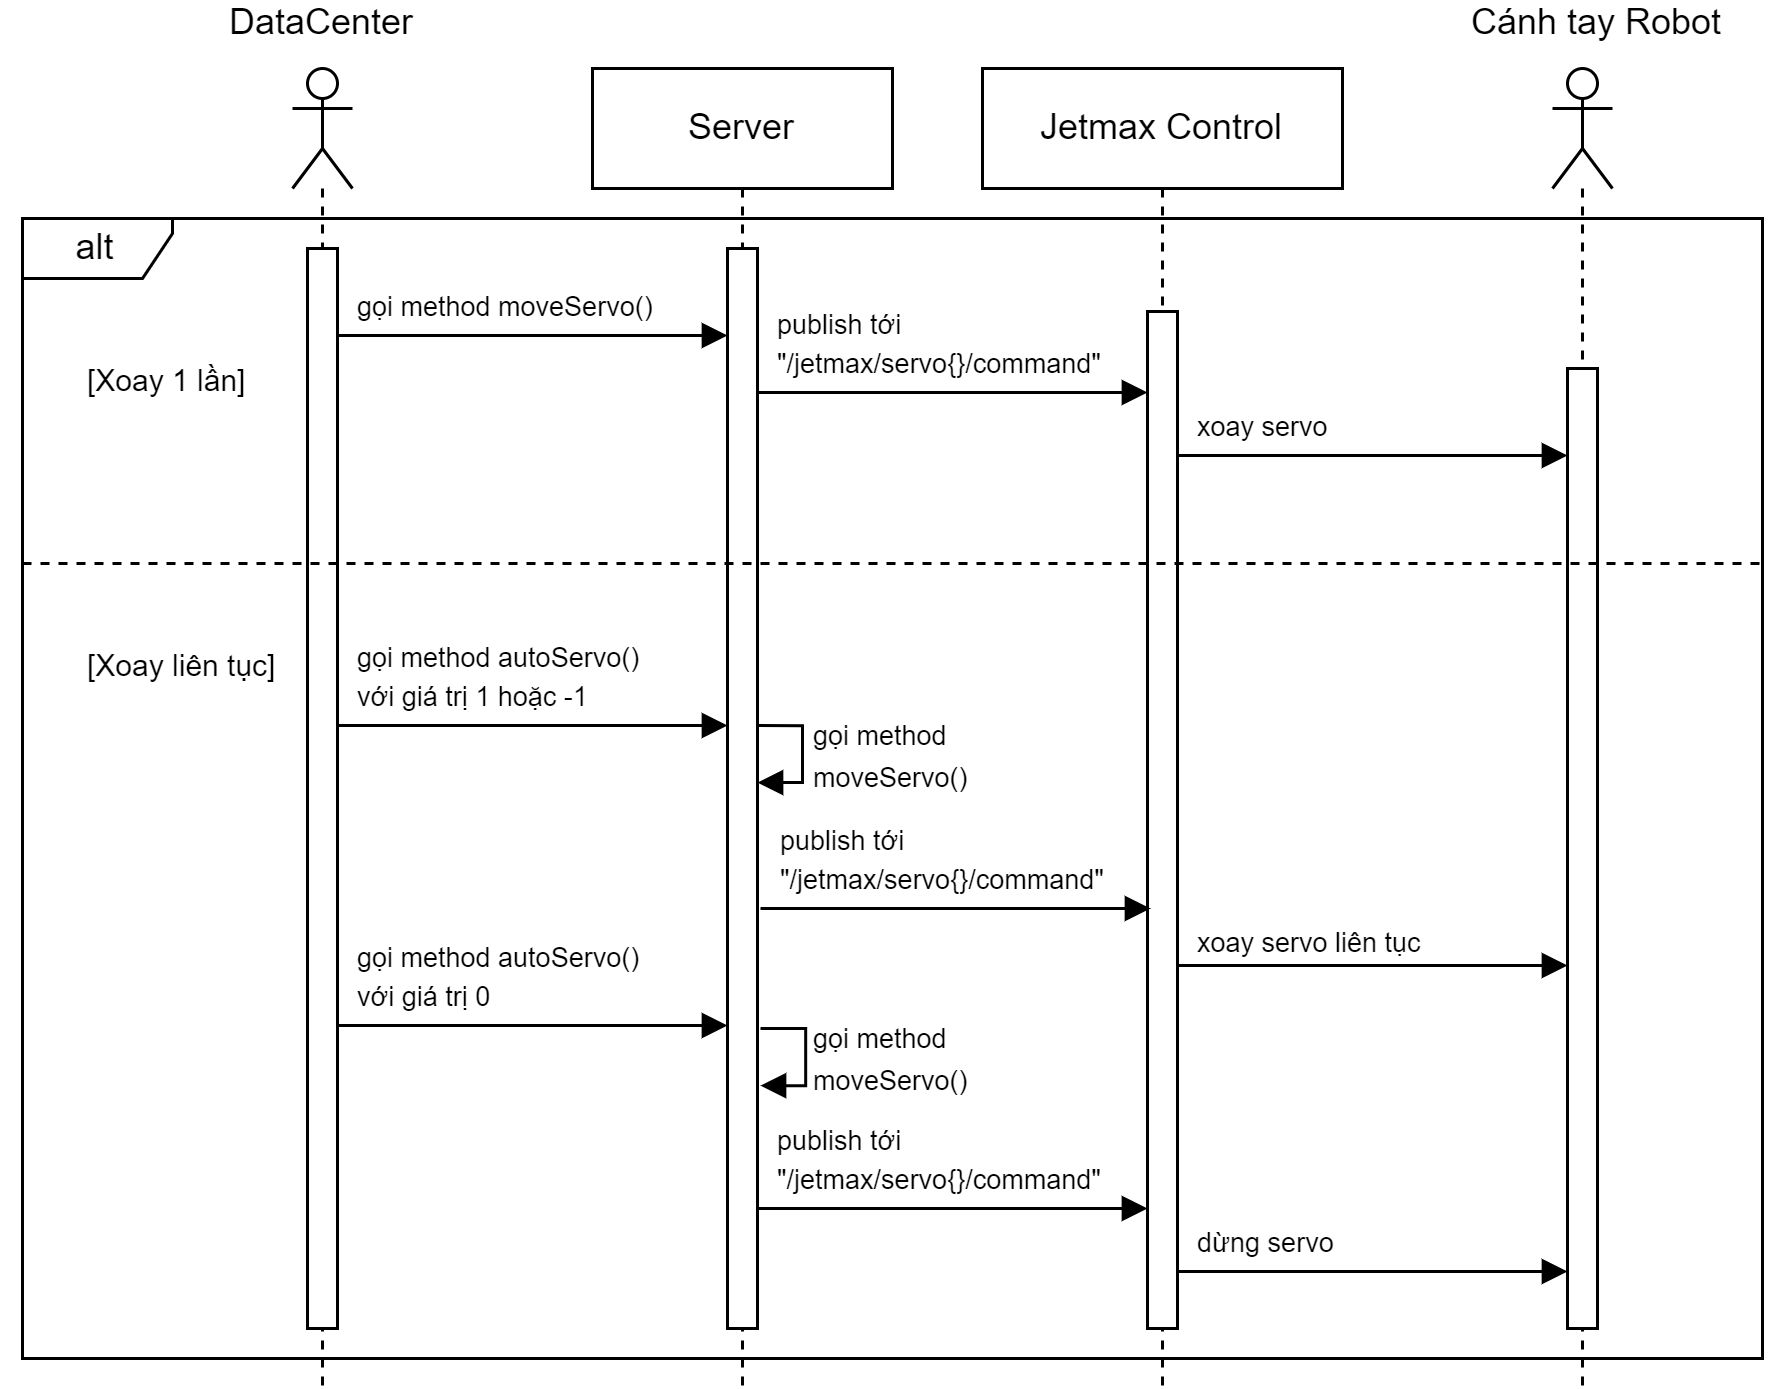
\includegraphics[width=0.8\textwidth]{Images/Implementation/Control/dieukhientheo_servo.jpg}
        \caption{Sequence diagram của điều khiển theo servo}
    \end{figure}

    
    
    \item \textbf{Điều khiển cánh tay theo tọa độ:} Tương tự như điều khiển bằng servo thì ở tính năng này method mà Server cung cấp có tên là \textbf{moveCordinate}, Server sẽ publish vào topic ROS có tên là "/jetmax/relative\_command" với tham số truyền vào là một message chứa ba tọa dộ x, y, z. Bên dưới Jetmax Control thực thi bằng cách lấy tọa độ hiện tại và cộng vào tọa độ được truyền vào (relative). Dưới đây là sequence diagram của chức năng này:
    \begin{figure}[!h]
        \centering
        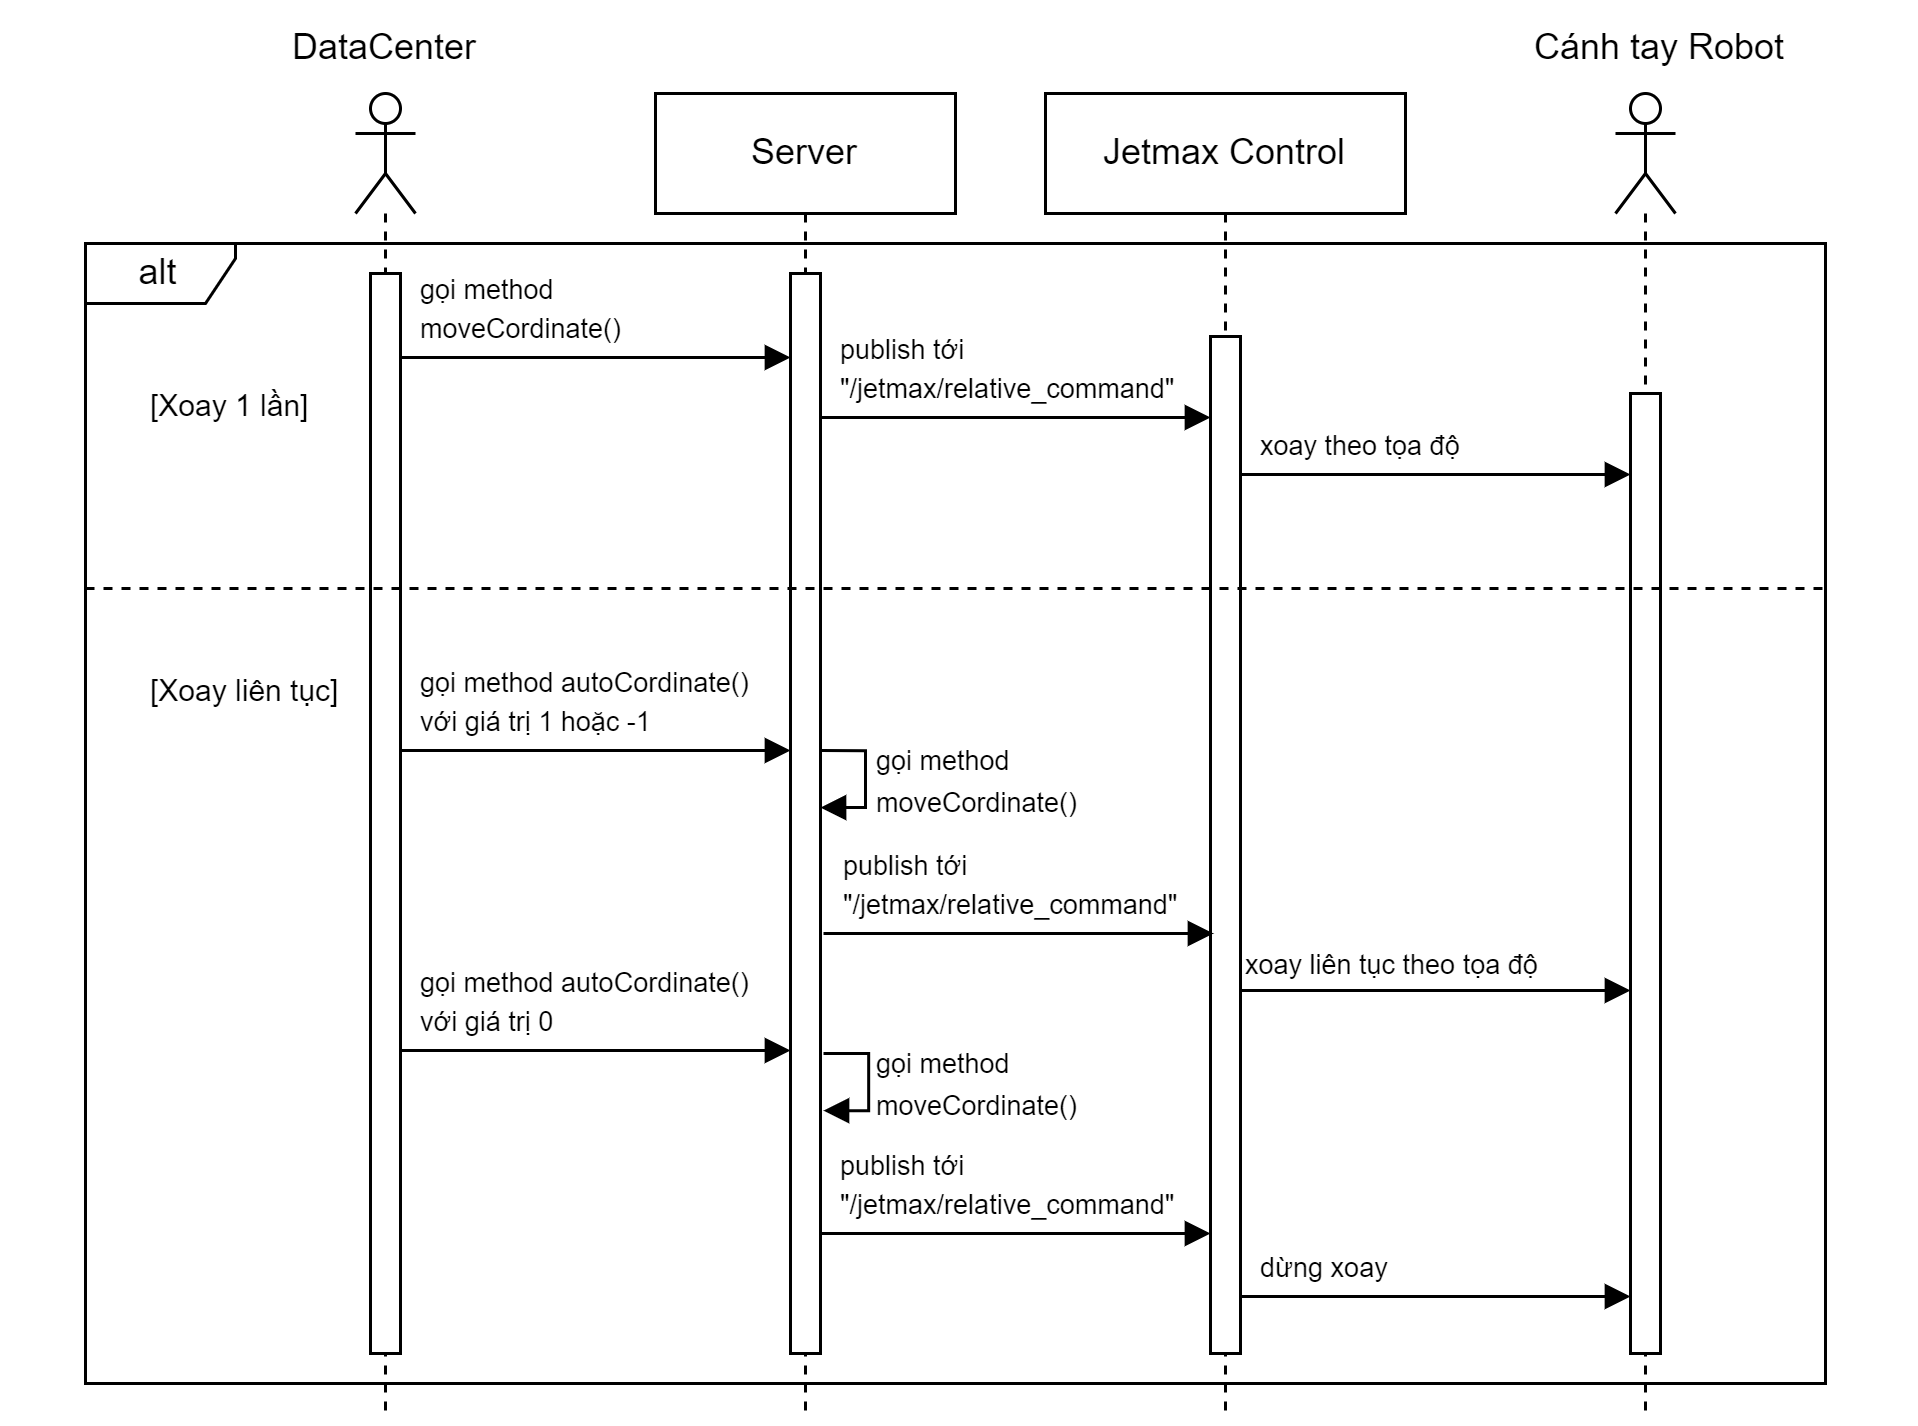
\includegraphics[width=0.8\textwidth]{Images/Implementation/Control/dieukhientheo_toado.jpg}
        \caption{Sequence diagram của điều khiển theo tọa độ}
    \end{figure}

    \newpage
    
    \item \textbf{Thay đổi tốc độ xoay:} Để thay đổi tốc độ xoay của các servo, Server OPC cung cấp method có tên là \textbf{changeSpeed}, khi method được gọi, phía Server sẽ lưu tốc độ này vào 1 biến toàn cục. Biến này sẽ được đính kèm vào các message khi gọi tới các topic ROS kiểm soát chuyển động cánh tay. Bên dưới là sequence diagram của chức năng:
    \begin{figure}[!h]
        \centering
        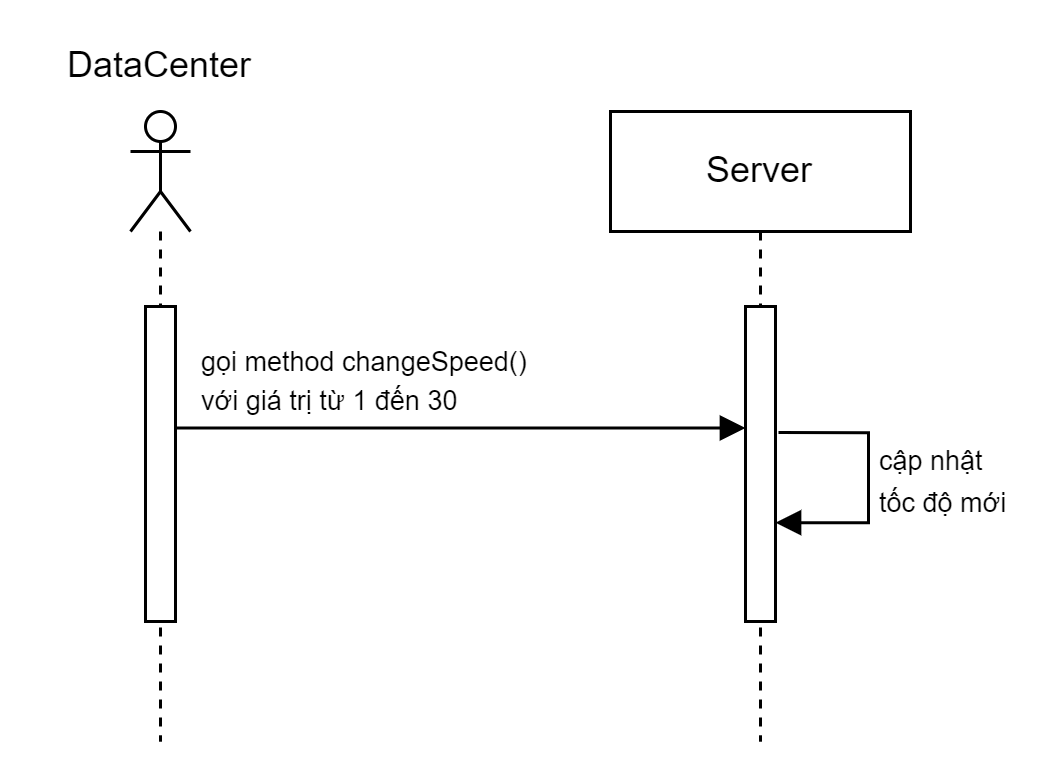
\includegraphics[width=0.6\textwidth]{Images/Implementation/Control/changespeed.jpg}
        \caption{Sequence diagram của thay đổi tốc độ xoay}
    \end{figure}
    
    \item \textbf{Về vị trí ban đầu:} Đây là chức năng đưa cánh tay về 1 vị trí mặc định đã được chọn trước, ở vị trí này cánh tay sẽ có tọa độ là \{x = 0,y = -162.9, z = 212.8\} và gốc các servo mid=500,left=500,right=500, các giá trị khác tương ứng gripper=90, rotator=90. Method này có tên là \textbf{goHome}; khi gọi tới method, Server sẽ thực thi việc gọi tới service ở topic ROS có tên là "/jetmax/go\_home" với một message rỗng ( Empty ). Dưới đây là sequence diagram cho chức năng:
    \begin{figure}[!h]
        \centering
        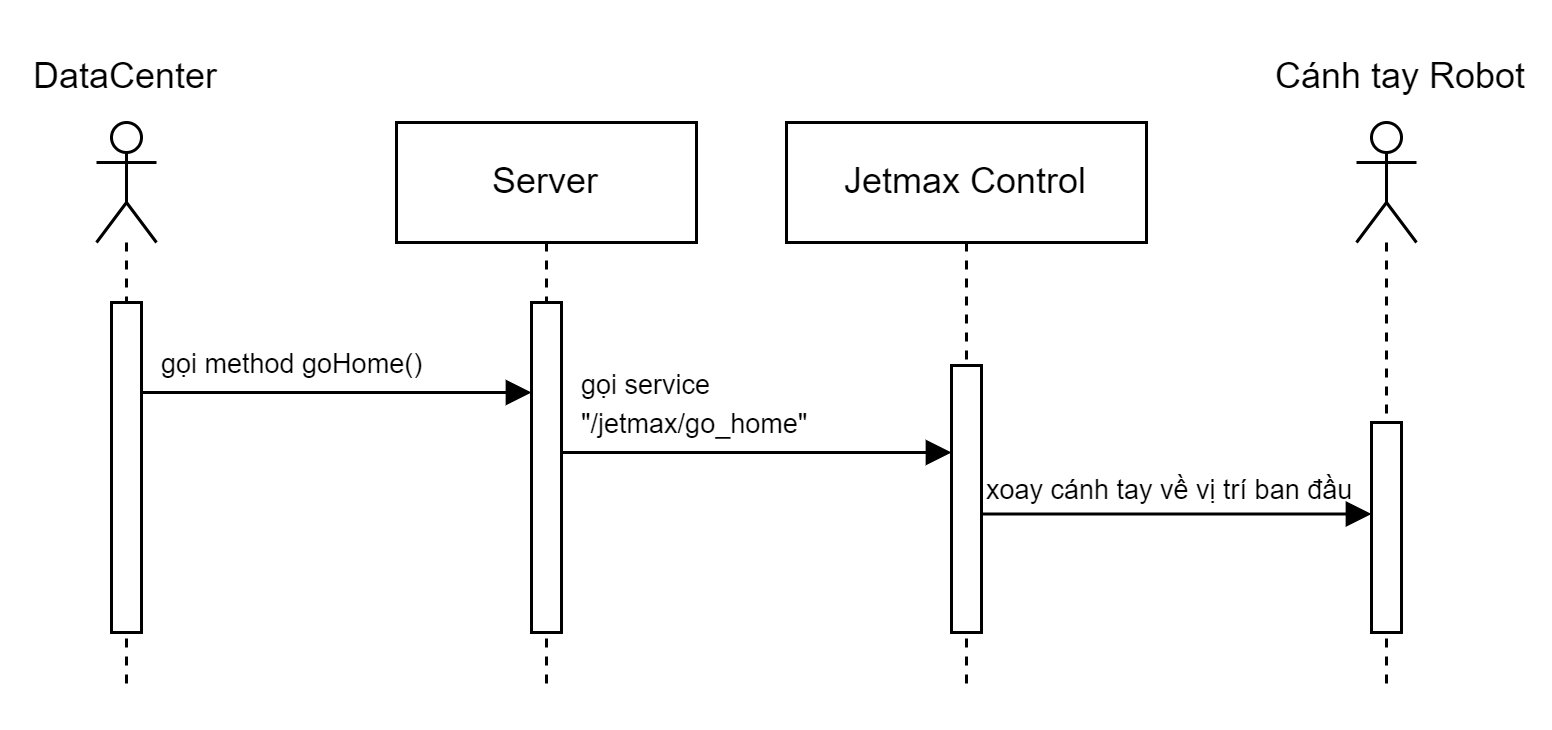
\includegraphics[width=0.8\textwidth]{Images/Implementation/Control/goHome.jpg}
        \caption{Sequence diagram của về vị trí ban đầu}
    \end{figure}
    
    \item \textbf{Bật tắt sucker:} Để bật hoặc tắt máy hút được gắn ở đầu của cánh tay, Server cung cấp một method có tên là \textbf{sucker}. Khi được gọi Server sẽ thực hiện publish một message có giá trị là TRUE hoặc FALSE vào topic ROS có tên "/jetmax/end\_effector/sucker/command". Dưới đây là sequence diagram của chức năng:
    \begin{figure}[!h]
        \centering
        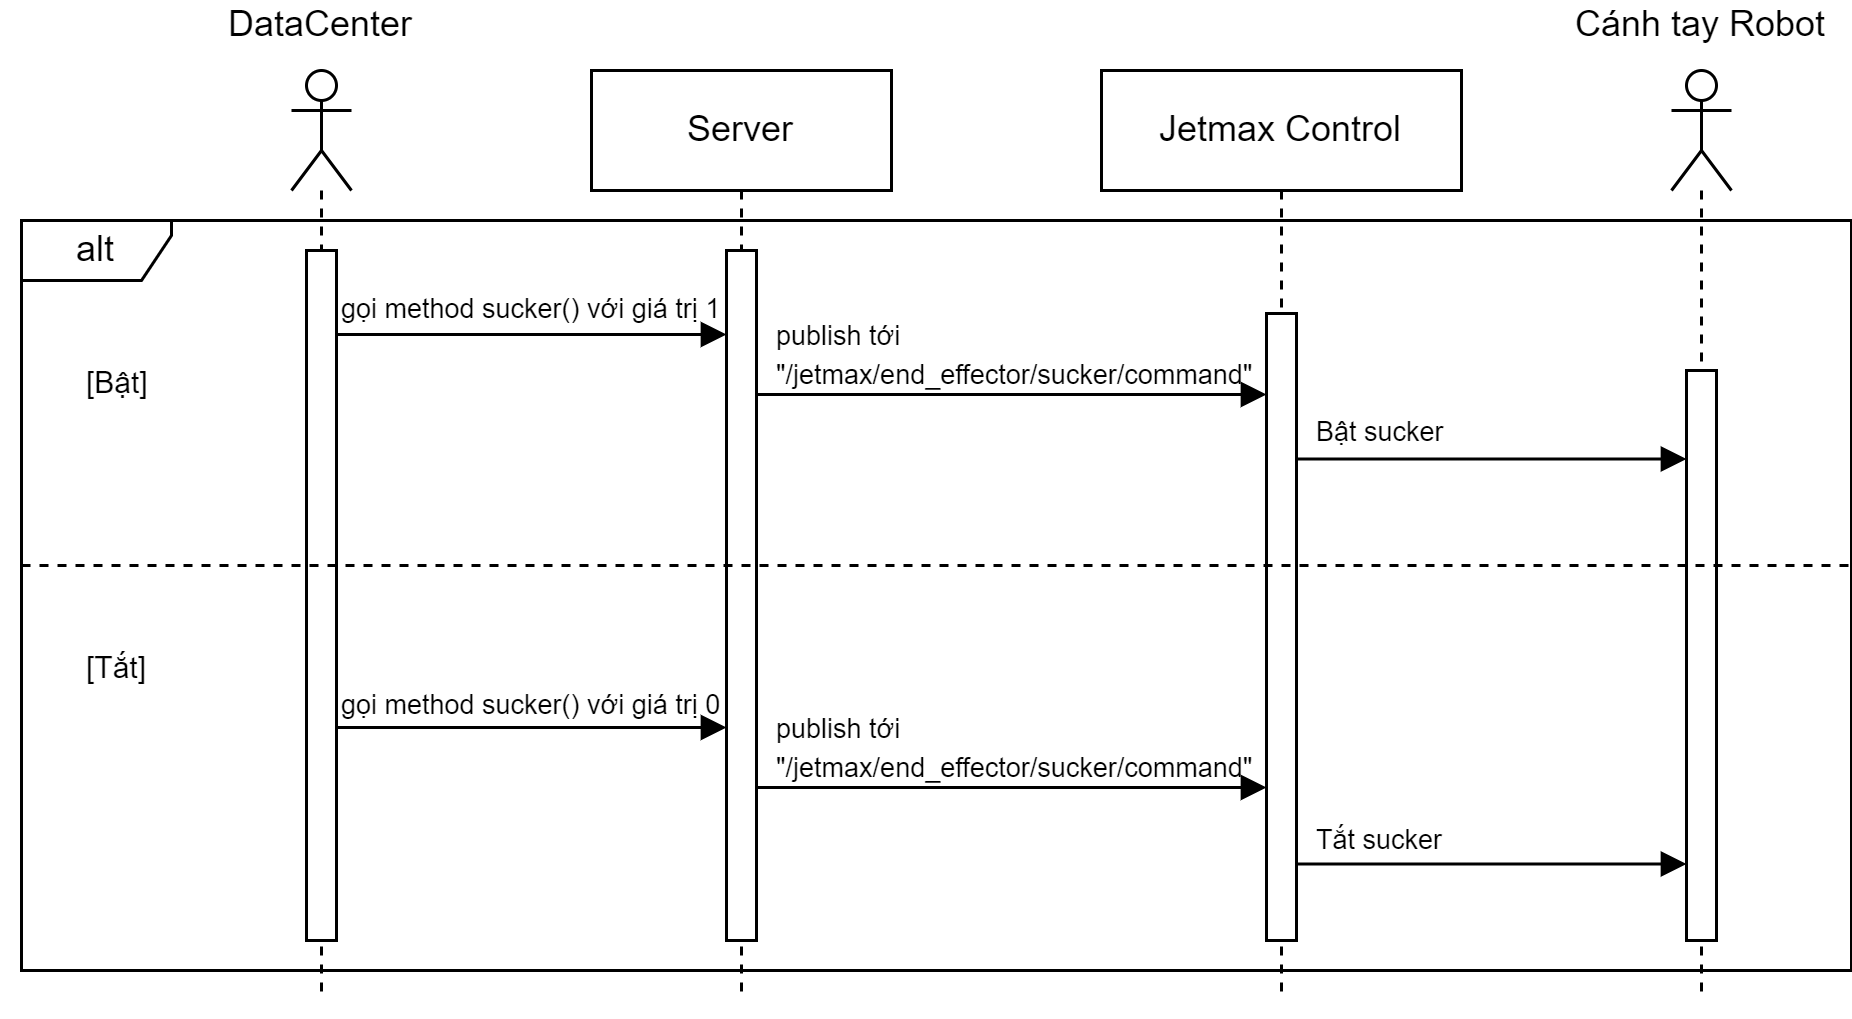
\includegraphics[width=0.8\textwidth]{Images/Implementation/Control/sucker.jpg}
        \caption{Sequence diagram của bật tắt sucker}
    \end{figure}
    
    \item \textbf{Đưa cánh tay tới tọa độ:} Khác với chức năng điều khiển theo servo, ở chức năng này cánh tay sẽ di chuyển tới một vị trí nhất định thay vì dùng lại tọa độ cũ cộng vào tham số. Server cung cấp method \textbf{setCordinate} để thực hiện chức năng này, khi được gọi Server sẽ thực hiện publish 1 message chứa tọa độ \{x, y, z\} vào topic ROS "/jetmax/command", khi nhận được tín hiệu cánh tay sẽ lập tức di chuyển đến toạ độ mới có giá trị là \{x, y, z\}. Bên dưới là sequence diagram của chức năng:
    \begin{figure}[!h]
        \centering
        \includegraphics[width=0.8\textwidth]{Images/Implementation/Control/setCordinate.jpg}
        \caption{Sequence diagram của đưa cánh tay tới tọa độ}
    \end{figure}
    
    \item \textbf{Kich hoạt AI xếp gỗ:} Cánh tay jetmax được tích hợp một số dịch vụ AI kèm theo, trong đó tiêu biểu là chức năng sắp xếp các khối gỗ theo thứ tự và theo dõi vật thể với màu sắc cụ thể. Để kích hoạt tính năng sắp xếp khối gỗ, bước đầu tiên chúng ta gọi tới method có tên \textbf{AIservice} được cung cấp trong Server OPC, truyền vào đó tên của chức năng và tham số thứ 2 là một biên boolean với giá trị TRUE nếu kich hoạt hoặc FALSE để thoát khỏi chức năng này. Khi method được gọi Server dựa vào giá trị được gửi đến, sau đó thực hiện gọi tới một service với topic ROS có tên là "/\{service\_name\}/enter"; ở đây service\_name là tên của dịch vụ AI tức "palletizing". Tiếp theo để AI chạy, chúng ta cần gọi tới method \textbf{AIserviceRun} truyền vào đó tên của dịch vụ ở đây chúng ta sử dụng "palletizing", Server sẽ tiếp tục thực hiện gọi 1 service khác có tên là "/\{service\_name\}/set\_running". Sau đó AI sẽ hoạt động cánh tay sẽ tìm và sắp xếp các khối gỗ theo thứ tự của id. Để thoát khỏi AI này ta gọi tới method ban đầu và truyền vào đó giá trị FALSE. Bên dưới là sequence diagram của chức năng kích hoạt/thoát AI xếp gỗ.
    \begin{figure}[!h]
        \centering
        \includegraphics[width=0.8\textwidth]{Images/Implementation/Control/palletizing.jpg}
        \caption{Sequence diagram của kích hoạt AI xếp gỗ}
    \end{figure}

    \newpage
    
    \item \textbf{Kich hoạt AI theo dõi màu:}AI này được phát triển trên thư viện OpenCV, dùng trong việc nhận diện màu sắc của khối vật thể. Tương tự như sắp xếp khối gỗ, để kích hoạt theo dỗi khối màu lần lượt gọi tới các method sau:
    \begin{itemize}
        \item \textbf{AIservice}: Để kích hoạt AI với tên truyền vào là "object\_tracking",giá trị boolen kèm theo là TRUE.
        \item \textbf{AIsetTarget}: Tiếp theo để set màu của khối object cần theo dõi, ta gọi method này với giá trị truyền vào là tên của AI "object\_tracking", màu tương ứng "red", "green", hoặc "blue".
        \item \textbf{AIserviceRun}: Cuối cùng để AI hoạt động thì phải gọi tới method này với các giá trị tương ứng.
    \end{itemize}
    Để thoát khỏi AI ta gọi tới \textbf{AIservice} với giá trị boolen là FALSE để thoát. Sau đây là sequence diagram cho chức năng này.
    \begin{figure}[!h]
        \centering
        \includegraphics[width=0.8\textwidth]{Images/Implementation/Control/object-tracking.jpg}
        \caption{Sequence diagram của kích hoạt AI theo dõi màu}
    \end{figure}

    \newpage
    
    \item \textbf{Kich hoạt AI phân loại rác:} Đây là tính năng mà nhóm đã phát triển, là sự kết hợp của các bài toán như: nhận diện màu bằng OpenCV, nhận diện vật thể thông qua kỹ thuật học có giám sát (supervised learning) được thực hiện trên mô hình YOLOv5. Cụ thể sẽ được trình bày ở phần sau.Để kích hoạt AI này, cần thực hiện gọi tới các method sau Server:
    \begin{itemize}
        \item \textbf{AIservice:} Gọi tới method này với giá trị truyền vào là "waste\_classification" và giá trị boolean kèm theo là TRUE.
        \item  \textbf{waste\_class:} Gọi tới method này để thiết lập loại rác mong muốn.

        \item  \textbf{AIserviceRun}: Để AI được khởi chạy, gọi method này với các tham số tương ứng.
        
        \item  \textbf{set\_suck\_waste}:Khi AI đã hoạt động, gọi method này với tham số truyền vào là các giá trị từ 1 đến 4, tương ứng cho các trạng thái của chức năng "tìm và gắp", "tìm và thả".     
    \end{itemize}
    Để thoát khỏi AI ta gọi tới \textbf{AIservice} với giá trị boolen là FALSE để thoát. Sau đây là sequence diagram cho chức năng này.
    \begin{figure}[!h]
        \centering
        \includegraphics[width=0.8\textwidth]{Images/Implementation/Control/waste-classification.jpg}
        \caption{Sequence diagram của kích hoạt AI phân loại rác}
    \end{figure}

    \newpage
    
    \item \textbf{Cập nhật trạng thái cánh tay:} Server sẽ luôn lắng nghe các giá trị trạng thái của canh tay thông qua các topic ROS mà khối Jetmax Control tạo ra, sau đó cập nhật liên tục các giá trị này lên các node, cung cấp cho người dùng trạng thái theo thời gian thực của thiết bị - cụ thể là cánh tay Jetmax. Các topic ROS được Server OPC lắng nghe gồm:
    \begin{itemize}
        \item \textbf{/jetmax/status:} Lây trạng thái tọa độ, góc servo của cánh tay, trạng thái đầu hút...
        \item  \textbf{/jetmax/AIEnterCurrent, /jetmax/AIRunCurrent, /jetmax/AIColorCurrent}: Lấy thông tin của chức năng AI hiện tại đang hoạt động trên cánh tay.
        \item \textbf{/waste\_classification/set\_suck, /waste\_classification/\\
        set\_waste\_class:} Lây thông tin chi tiết của AI phân loại rác.
        \item \textbf{/usb\_cam/image\_rect\_color:} Lấy dữ liệu hình ảnh mặc định từ usb camera tích hợp trên cánh tay Jetmax. 
        \item \textbf{/{topic}/image\_result:} Lấy dữ liệu ảnh đã được xử lý trong các chức năng AI khi các chức năng AI này được kích hoạt. Dữ liệu hình ảnh sẽ được lấy từ topic này thay vì topic mặc định usb\_cam
    \end{itemize}
    Những dữ liệu này sau khi lắng nghe sẽ được cập nhật vào các node tương ứng trên Server OPC. Ngoài ra, nhóm cũng thực hiện gửi dữ liệu ảnh thu được từ camera lên node OPC UA của Server. Tuy nhiên, vì dữ liệu ảnh khá lớn (kích thước 640 * 480 * 3 = 921600 byte cho từng tấm ảnh),Server OPC UA không thể xử lý và gửi toàn bộ lượng dữ liệu đó với tốc độ nhanh, liên tục. Chính vì thế, riêng đối với dữ liệu ảnh, nhóm đã phải sử dụng giải thuật nén của thư viện PIL (Python Imaging Library) và thư viện OpenCV để nén ảnh lại xuống còn khoảng 8900 bytes, đánh đổi giảm bớt kích thước ảnh và chất lượng ảnh nhằm tăng khả năng đáp ứng của Server. Dưới đây là sequence diagram cho chức năng này: 
    \begin{figure}[!h]
        \centering
        \includegraphics[width=0.8\textwidth]{Images/Implementation/Control/update-state.jpg}
        \caption{Sequence diagram của cập nhật trang thái cánh tay}
    \end{figure}
\end{itemize}


\newpage

\section{Tính năng AI: Phân loại rác thải bán tự động}

Một trong những vấn đề lớn nhất của thế giới hiện nay là ô nhiễm môi trường. Nhiều nỗ lực đã được thực hiện để giảm thiểu ô nhiễm, và trong đó việc phân loại rác đóng vai trò quan trọng. Tuy nhiên, phân loại rác thủ công có thể là một quá trình phức tạp và tốn thời gian. Để giải quyết vấn đề này, công nghệ trí tuệ nhân tạo (AI) đã được sử dụng để xây dựng các hệ thống phân loại rác tự động. Trong đồ án này, nhóm đã thiết kế và hiện thực chức năng phân loại rác bán tự động dựa trên AI, với hy vọng đóng góp một phần nhỏ vào việc giảm thiểu ô nhiễm môi trường.

Tính năng phân loại rác thải đã và đang được nghiên cứu trong khá nhiều bài báo. Vào năm 2016, Williams và Bentil \cite{williams2016design} giới thiệu và hiện thực một hệ thống tự động sắp xếp rác thải sử dụng vi điều khiển, và đã thành công phân loại rác thải hữu cơ và rác thải vô cơ sử dụng cảm biến khí gas. Paulraj \cite{gundupalli2016automated} đề xuất giải thuật để nhận biết rác thải trên hình ảnh chụp được từ camera nhiệt. Tác giả cũng xây dựng một cánh tay robot 5 bậc tự do tích hợp camera nhiệt, cảm biến khoảng cách để thực hiện phân loại rác. Sadia Zahin Diya \cite{diya2018developing} trong nghiên cứu vào năm 2018, xây dựng một hệ thống phân loại rác thải thông minh với mục tiêu phù hợp trong bối cảnh quốc gia Bangladesh. Trong nghiên cứu của mình, tác giả xây dựng hệ thống điều khiển và phân loại rác có khả năng nhận biết rác thải kim loại, hữu cơ và nhựa sử dụng các cảm biến IR (Infrared Ray), cảm biến từ trường và cảm biến hiệu điện thế. Các nghiên cứu đều thử nghiệm với rác thải thực tế, tuy nhiên chỉ có thể phân loại một số loại rác cố định.


Về phía nhóm, việc thực hiện tính năng AI phân loại rác không phải là mục tiêu chính của đề tài, nhưng đây là một chức năng sáng giá để thể hiện khả năng điều khiển thiết bị thông qua OPC UA. Nhà phát triển cánh tay JetMax - Hiwonder đã cung cấp sẵn cho cánh tay robot chức năng phân loại rác tự động, tuy nhiên không phải là rác thực tế mà chỉ là ảnh các rác thải được in lên một tấm thẻ hình vuông. Các rác thải buộc phải đặt ngay phía trước cánh tay khi cánh tay ở vị trí mặc định để nhận dạng, và khi nhận diện được rác thải, sẽ tự động mang rác tới một vị trí được chỉ định. Vì những giới hạn này, nhóm quyết định nâng cấp tính năng phân loại rác này thành "phân loại rác bán tự động" hoạt động theo máy trạng thái. Về khái niệm "bán tự động", khi này nhóm có thể tự do đặt rác thải ở một nơi khác và điều khiển cánh tay thủ công tới để tự động hút lên bằng AI. Sau khi hút, nhóm lại điều khiển cánh tay thủ công tới khu vực thùng rác, và để cánh tay tự nhận diện loại thùng rác cần bỏ rác vào. Việc nhận diện rác thải và thùng rác được thực hiện bằng cách phân tích ảnh chụp từ USB camera và các thuật toán AI đã được huấn luyện sẵn có trong cánh tay JetMax. Vì giới hạn về thời gian và điều kiện, nhóm vẫn thực hiện nhận dạng rác thải dưới dạng các thẻ vuông để dễ dàng hút bằng đầu hút của cánh tay JetMax.

\subsection{Yêu cầu hệ thống}

Phần tiếp theo, nhóm đề ra một số yêu cầu chức năng và phi chức năng cho tính năng AI phân loại rác thải, để làm rõ hoạt động mong đợi và khả năng của tính năng này.

\subsubsection{Yêu cầu phi chức năng}


Các yêu cầu phi chức năng cho tính năng này được nhóm đặt ra như sau:
\begin{itemize}
    \item Chức nằng này phải đảm bảo độ chính xác và đáng tin cậy trong việc phân loại các loại rác khác nhau, từ đó giúp người dùng phân biệt dễ dàng và đúng đắn.
    \item Hệ thống phân loại rác cần được thiết kế để có thể mở rộng trong tương lai, khi có thêm các loại rác mới cần phân loại.
    \item Tính năng phân loại rác cần được thiết kế để tương tác dễ dàng và trực quan với người dùng, giúp họ sử dụng một cách thuận tiện và hiệu quả.
    \item Độ trễ phản hồi của tính năng không quá 1 giây
\end{itemize}
\subsubsection{Yêu cầu chức năng}
Các yêu cầu về chức năng cho tính năng phân rác bán tự động như sau:
\begin{itemize}
    \item Nhận diện được loại rác cụ thể và xác định được vị trí của nó.
    \item Nhận diện được loại thùng rác tương ứng với từng loại rác và vị trí của nó
    \item Người dùng có thể điều khiển qua lại để đưa camera bắt được hình ảnh của rác hoặc thùng rác.
    \item Xác định vùng hoạt động tốt cho camera
    \item Thao tác hút hoặc thả trên cùng một phím nhấn.
\end{itemize}
\subsection{Sơ đồ use case diagram}
Dựa vào những yêu cầu phi chức năng và chức năng mà nhóm xem xét bên trên, nhóm đưa ra một use case đơn giản cho chức năng Phân loại rác bán tự động như hình.

    \begin{figure}[!h]
        \centering
        \includegraphics[width=0.8\textwidth]{Images/Implementation/AI/waste_usecase.jpg}
        \caption{Use case diagram của phân loại rác bán tự động}
    \end{figure}



Người dùng sẽ tương tác với chức năng phân loại rác bán tự động này bằng VR app được nhóm phát triển trên Unity3D và chạy trên Oculus, ứng dụng gửi nhận dữ liệu từ cánh tay thông qua module trung gian Datacenter, sẽ được giới thiệu ở phần tiếp theo. Cánh tay và chức năng AI sẽ được quản lý bởi máy tính nhúng Jetson Nano chứa một server OPC trên đó.
\subsection{Hiện thực chức năng phân loại rác bán tự động}
Chức năng được nhóm hiện thực dựa trên hai thư viện nổi tiếng là OpenCV và YOLOv5, trong chức năng này nhóm chia ra làm hai chức năng nhỏ cần hiện thực.

\begin{itemize}
    \item Thứ nhất, nhóm sử dụng kỹ thuật học có giám sát ( supervise learning ) để train cho mô hình AI nhận diện các loại rác. Ở chức năng này nhóm sử dụng thư viện YOLOv5 trên python để train data cho mô hình. Khi camera dò được thẻ rác nào đó, mô hình sẽ trả về các thông tin như tên rác, loại rác và vị trí của vật thể so với đầu hút. Từ những thông tin đó, AI sẽ tính toán và đưa ra vị trị tương ứng để đưa đầu hút của cánh tay tới vị trí của mảnh rác và hút nó.
    \item Thứ hai, nhóm sử dụng chức năng nhận diện màu sắc được tích hợp trong thư viện OpenCV để nhận diện những loại thùng rác. Sau khi hút rác, người dùng sẽ di chuyển cánh tay sao cho camera nhìn thấy các thùng rác, AI sẽ tự động chọn thùng phù hợp với loại rác hiện tại và thả và đó. Cũng tương tự như quá trình tìm và nhận diện rác, quá trình nhận diện loại thùng rác cũng sẽ trả về các thông tin như loại rác, vị trí của thùng đó so với đầu hút. Dựa vào đó ta sẽ tìm được vị trí so với cánh tay và thả rác vào đó.
\end{itemize}

Chức năng sẽ có 4 trạng thái chính, được mô tả như sau:
    \begin{figure}[!h]
        \centering
        \includegraphics[width=0.8\textwidth]{Images/Implementation/AI/state-machine_1.jpg}
        \caption{Sơ đồ máy trạng thái của chức năng}
    \end{figure}
\begin{itemize}
    \item \textbf{IDLE:} Đây là trạng thái đầu tiên khi chức năng được khởi động, ở trạng thái này camera sẽ cung cấp hình ảnh cho AI nhận diện rác thải và đợi một event trigger từ người dùng, nếu phát hiện được rác thuộc loại cần phân loại, AI sẽ vẽ một khung hình chữ nhật bao quanh loại rác đó và kèm theo nhãn của loại rác. Khi nhận event trigger từ người dùng chức năng chuyển sang trạng thái thứ 2 SUCK.
    \item \textbf{SUCK:} Ở trạng thái AI sẽ cung cấp vị trí của vật thể gần nhất so với camera, để di chuyển chính xác ta cần vị trí của vật thẻ so với cánh tay, vị trị này sẽ có được sau khi qua một vài bước tính toán và sẽ được trình bày trong phần tiếp theo. Sau khi tính được vị trí cần đến, cánh tay sẽ di chuyển, hút vật thể, đi lên theo chiều Z và chuyển sang trạng thái HOLD.
    \item  \textbf{HOLD:} Ở trạng thái này, camera sẽ nhận diện thùng rác dựa vào màu sắc được thiết lập trước đó, tương ưng cho từng loại rác, ở trạng thái này người dùng sẽ di chuyển cánh tay qua lại để tìm được vị trí của thùng rác, khi xác định được vị trí và nhận event trigger sẽ chuyển sang trạng thái tiếp theo RELEASE.
    \item \textbf{RELEASE:} Khi xác định được vị trí của thùng rác so với camra, cũng tương tự sẽ tinh toán như ở trạng thái SUCK, tìm ra vị trị so với cánh tay, cánh tay sẽ di chuyển đến thả vật thể và quay về trạng thái IDLE.
\end{itemize}
\subsubsection{Xác định vị trí của vật thể so với cánh tay}
Ở hai trạng thái \textbf{SUCK} và \textbf{RELEASE}, các mô hình AI trả về cho ta một tọa độ vị trí của vật thể gần nhất, tuy nhiên đây là tọa độ của vật thể so với camera, để cánh tay đến được vật thể thì phải qua một bước tính toán, chuyển từ tọa độ so với camera thành tọa độ so với cánh tay.
\begin{figure}[!h]
    \centering
    \includegraphics[width=0.6\textwidth]{Images/Implementation/AI/AI_math_1.jpg}
    \caption{Mô tả bài toán}
\end{figure}

Trong hình bên trên O là góc tọa độ cánh tay, O' là gốc tọa độ của camera, AI sẽ cung cấp cho ta tọa độ vật thể A trong tọa độ x'O'y', chúng ta cần chuyên tọa độ này thành tọa độ mời trong hệ xOy. Nhóm giải quyết qua hai bước sau:
\begin{itemize}
    \item Tìm góc tạo bởi vật thể A (OA) và trục Oy của cánh tay, sau đó xoay servo mid theo góc tìm được lúc ta có O, O', A thẳng hàng. Sau đó chuyển sang bước tiếp theo.
    
    \begin{figure}[!h]
        \centering
        \includegraphics[width=0.6\textwidth]{Images/Implementation/AI/AI_math_2.jpg}
        \caption{Sau khi xoay cánh tay theo gốc alpha}
    \end{figure}

    \item  Công thức tính gốc xoay \[\angle alpha = arctan( \frac{x'}{OO'+y'} ) \] 
     
    \item Sau khi xoay servo mid của cánh tay theo góc tìm được ở bước một, ta có O, O', A thẳng hàng, tìm được độ dài của OA, OO' và có được tọa độ điểm O' trong xOy, dựa vào biểu thức vector: OA = alpha*OO', trong đó ta tìm được alpha theo biểu thức độ dài, từ đó ta suy ra được tọa độ điểm A trong hệ tọa độ xOy.
\end{itemize}

Sau khi tìm được vị trí điểm A cánh tay sẽ di chuyển tới tọa độ đó và thực hiện thao tác hút/thả với vật thể.

\subsubsection{Sequence diagram của chức năng}

Trong phần tiếp theo sau đây, nhóm sẽ trình bày cụ thể hơn về sơ đồ mô tả cách thức hoạt động của chức năng.

\begin{figure}[!h]
    \centering
    \includegraphics[width=0.9\textwidth]{Images/Implementation/AI/AI-sequence.png}
    \caption{Sequence diagram của chức năng}
\end{figure}

Quan sát sequence diagram, ta có thể nói chi tiết hoạt động của chức năng như sau:
\begin{itemize}
    \item Khi AI được khởi động, chương trình sẽ thiết lập loại rác tương ứng mà người dùng nhập vào, lúc này chức năng sẽ nằm ở trạng thái IDLE, ở trạng thái này camera sẽ nhận diện được những mãnh rác thuộc loại rác mà người dùng đã thiết lập, hình ảnh cùng các trạng thái sẽ liên tục được cập nhật vào OPC server thông qua các node của ROS.
    Lúc này người dùng sẽ xoay các servo để đưa các mãnh rác vào vùng nhận diện của camera.
    \item Sau khi nhận diện và phát hiện vật thể tương ứng, người dùng sẽ kích hoạt một event gắp rác, lúc này trạng thái của chức năng sẽ chuyển sang SUCK, ở trạng thái này, AI sẽ tính toán lại tọa độ, đưa đầu hút đến tọa độ đó và hút, sau khi hút xong cánh tay sẽ di chuyển lên trên và chuyển sang trạng thái HOLD, trong quá trình này, người dùng không cần thao tác vào cánh tay cho đên khi cánh tay dừng lại và chờ event tiếp theo được kích hoạt
    \item Ở trạng thái HOLD người dùng sẽ di chuyển cánh tay đưa thùng rác tương ứng vào vùng nhận diện của camera, lúc này camera sẽ nhận diện thùng rác theo màu tương ứng với loại ra mà người dùng thiết lập, người dùng sẽ xoay cánh tay để đưa thùng rác vào vùng nhận diện của camera để tiến hành phân loại.
    \item  Khi nhận diện được thùng rác, người dùng kích hoạt một event để thả rác vào thùng, khi event được kích hoạt, chức năng sẽ chuyển sang trạng thái RELEASE, ở trạng thái này AI sẽ tính toán lại tọa độ, đưa cánh tay đến tọa độ mới và thả vật thể đang hút ra. Sau khi thả cánh tay sẽ di chuyển lên trên và chuyển sang trạng thái ban đầu tức IDLE, trong quá trình này, người dùng không cần thao tác vào cánh tay cho đến khi cánh tay dừng lại và chờ event tiếp theo được kích hoạt.
\end{itemize}
 
\section{Module Datacenter}
% mô tả về datacenter

% Như đã trình bày ở phần kiến trúc hệ thống tổng quát, Datacenter là một module trung gian giữa module Control và module VR application. Sự kết hợp của Datacenter giúp cho ta có thể mở rộng mô hình điều khiển trong tương lai, khi có thể kết nối nhiều OPC server hơn vào Datacenter, để Datacenter tổng hợp dữ liệu, và sau đó ứng dụng VR có thể truy cập vào 1 điểm duy nhất là Datacenter để thực hiện điều khiển nhiều thiết bị một cách tiện lợi.

% Hiện tại, do giới hạn về tài nguyên và thiết bị, Datacenter chỉ đang kết nối với 1 OPC server của \textbf{module Control} nhằm điều khiển cánh tay. Khi chạy module Datacenter, nó sẽ tiến hành tạo kết nối với server OPC chạy trong module Control, sau đó "sao chép" - tạo ra những node và method bản sao lên Datacenter. 

Datacenter, hay có thể hiểu là một module với vai trò tập trung dữ liệu vào một điểm duy nhất nhằm xử lý, đồng bộ hoặc trở thành một gateway cho liên kết với cloud server hoặc ứng dụng từ xa. Việc sử dụng một module tập trung dữ liệu cũng giảm bớt độ phức tạp giữa các kết nối và giao tiếp, đặc trưng là khi người dùng chỉ cần kết nối tới module này là đủ để thu thập toàn bộ thông tin cần biết mà không cần phải đào sâu vào từng vị trí cụ thể. Đối với OPC UA, kể từ khi ra mắt, đã có nhiều nghiên cứu nhằm đề xuất một kiến trúc mang tính mở rộng dành cho OPC UA, hỗ trợ thu thập dữ liệu từ nhiều OPC UA server tại một nơi thay vì kiến trúc 1 client - 1 server mặc định. Fembach \cite{fernbach2014opc} giới thiệu một kiến trúc đa tác nhân (multi-agent) trong nghiên cứu gồm hai lớp OPC UA server. Lớp đầu tiên gồm 2 OPC UA server được cài đặt ở hai vị trí khác nhau để quan sát dữ liệu, và cả hai server này đều báo cáo dữ liệu tới một server OPC UA tổng hợp trên lớp thứ hai thông qua mạng không dây. Haskamp \cite{haskamp2018implementing} giới thiệu một kiến trúc khác nhằm nâng cấp các PLC truyền thống trở nên phù hợp với nền công nghiệp 4.0 tận dụng giao thức OPC UA. Các PLC chạy OPC server đều sẽ gửi dữ liệu lên dataFEED OPC Suite - một OPC UA server trung gian. Dữ liệu gửi lên đây cũng được dùng để gửi lên dịch vụ đám mây Microsoft Azure, từ đó có thể truy xuất, thu thâp bởi các ứng dụng quan trắc, điều khiển từ xa khác. Ahmad Abdelsattar \cite{abdelsattaropcgateway} đề xuất một khối gọi là Client/Gateway Node, gồm một OPC UA client có nhiệm vụ trung tâm thu thập thông tin từ các OPC server khác chạy trên PLC hoặc máy tính nhúng, nhằm cung cấp dữ liệu cho các ứng dụng nội bộ như Digital Twin, SCADA, hơn nữa cũng trở thành một gateway để giao tiếp với các dịch vụ đám mây thông qua các giao thức thông dụng TCP/IP hoặc UDP.


Trong đồ án này, nhóm cũng hiện thực kiến trúc với khối Datacenter - một module trung gian để tập trung dữ liệu nhằm giảm bớt sự phức tạp về hệ thống kết nối, vừa tạo khả năng mở rộng của hệ thống sau này. Trên Datacenter này sẽ có thể có nhiều OPC UA client, mỗi một client đảm nhiệm việc kết nối tới từng OPC UA server cần thu thập thông tin. Sau đó, các OPC UA client này sẽ cung cấp thông tin và dữ liệu cần thiết cho một OPC UA server chính chạy trên Datacenter, đóng vai trò trở thành điểm truy cập tập trung cho ứng dụng cần tiêu thụ dữ liệu. Hiện tại, hiện thực của nhóm chỉ bao gồm một OPC UA client để kết nối với OPC UA server bên module Control, và một OPC UA server chính trên Datacenter với khả năng tạo ra bản sao các node và method, cấu trúc dữ liệu giống hệt OPC server của module Control, đồng thời cập nhật liên tục theo thay đổi của module Control. Datacenter giờ trở thành khối tập trung và trung gian của dòng dữ liệu giữa ứng dụng và thiết bị thật.


% requirement
\subsection{Yêu cầu hệ thống}

Trước khi tiến hành hiện thực module Datacenter, ta cần đề ra những yêu cầu dành cho module này, về mặt phi chức năng và chức năng.

\subsubsection{Yêu cầu phi chức năng}

Các yêu cầu phi chức năng dành cho module Datacenter được đề ra:


\begin{itemize}
    \item Datacenter phải được thiết kế để độc lập với sự phát triển của module Control - Sự thay đổi của module Control gây ảnh hưởng ít hoặc không ảnh hưởng tới hiện thực của Datacenter
    \item Độ trễ cập nhật giá trị node trên Datacenter khi có sự thay đổi ở module Control không quá 1 giây
    \item Datacenter phải chịu được lượng kết nối vào lớn
    \item Datacenter được hiện thực có khả năng mở rộng thêm số lượng server OPC kết nối tới.
    \item Datacenter có khả năng hồi phục trong trường hợp mất kết nối tạm thời với server.
\end{itemize}

\subsubsection{Yêu cầu chức năng}

Các yêu cầu chức năng dành cho module Datacenter được đề ra:

\begin{itemize}
    \item Datacenter có thể browse các node trên OPC server được kết nối tới
    \item Datacenter có các variable node tự động cập nhật theo sự thay đổi của variable của server
    \item Datacenter tạo ra các method "bọc" gọi method tới server
    \item Datacenter cho phép người dùng tương tác với các node bằng cách kết nối tới OPC server đang chạy trong Datacenter.
    \item Datacenter sử dụng mã hóa dữ liệu 
\end{itemize}

% usecase
\subsection{Sơ đồ use case và máy trạng thái của chức năng}


Dựa vào các yêu cầu trên, ta có thể đưa ra use case đơn giản dành cho module Datacenter như hình. Phía bên các server sẽ kết nối với các sub client trong Datacenter, và sẽ được Datacenter browse rồi sao chép. Phía VR app có thể truy cập vào sub server trong Datacenter để điều khiển thông qua method hoặc theo dõi các node variable được "ánh xạ" từ các server.

\begin{figure}[H]
    \centering
    \includegraphics[width=0.7\textwidth]{Images/Implementation/Datacenter/Datacenter_usecase.jpg}
    \caption{Sơ đồ use case của Datacenter}
    \label{fig:use_case_Datacenter}
\end{figure}

% implementation

\subsection{Hiện thực module Datacenter}

Module Datacenter được nhóm hiện thực bằng ngôn ngữ Python, chạy trên Raspberry Pi 4 phiên bản 4GB. Để hiện thực OPC server và OPC client, thư viện \href{https://github.com/FreeOpcUa/opcua-asyncio}{github.com/FreeOpcUa/opcua-asyncio} được nhóm sử dụng. Đây là thư viện miễn phí, hiện thực OPC UA theo hướng bất đồng bộ (async), có cải tiến nhiều về tốc độ và chức năng và cú pháp so với thư viện \href{https://github.com/FreeOpcUa/python-opcua}{github.com/FreeOpcUa/python-opcua} trước đó. Sử dụng thư viện asyncua cũng giúp ta tận dụng được cú pháp async, await của python, từ đó giảm bớt vấn đề code bị "blocking" do gọi các hàm đồng bộ.

\subsubsection{Sơ đồ khối của module Datacenter}

Hiện tại, nhóm đã hiện thực được module Datacenter theo sơ đồ khối như sau:

\begin{figure}[H]
    \centering
    \includegraphics[width=0.7\textwidth]{Images/Implementation/Datacenter/Datacenter_block.jpg}
    \caption{Sơ đồ khối của Datacenter}
    \label{fig:blocks_Datacenter}
\end{figure}

Trong module hiện tại có 2 khối chính:

\begin{itemize}
    \item \textbf{Khối sub-server}: Khởi chạy 1 server OPC UA trên Datacenter, gồm các node và method là bản sao từ các server OPC UA mà khối sub-client kết nối tới. Khối này đảm nhận kết nối OPCUA của ứng dụng vào Datacenter.
    \item \textbf{Khối sub-client}: Khối đảm nhận việc kết nối tới một server OPC. Sau khi kết nối, khối này sẽ thực hiện việc browse (dò tìm) cấu trúc node cần quan tâm từ server OPC UA, sau đó tạo ra bản sao node và method lên khối sub-server. Đồng thời, khối sub-client này sẽ subscribe (đăng kí) theo dõi các node variable trên server OPC được kết nối tới, và nhận thông báo khi các node variable này thay đổi giá trị thông qua khối sub-handler.
    \begin{itemize}
        \item \textbf{\textit{Khối sub-handler}}: Kích hoạt khi nhận được thông báo có sự thay đổi giá trị của các node variable từ server OPC đang kết nối. Khối này sẽ xử lý nhằm cập nhật lại giá trị node variable tương ứng đang tồn tại trên sub-server. Hàm xử lý này được nhóm làm ngắn gọn để tránh tình trạng hàm xử lý "blocking" hoạt động chính của datacenter và gây tình trạng "hụt" xử lý gói tin.
    \end{itemize}
\end{itemize}

\subsubsection{Chi tiết một số chức năng}

Phần này sẽ liệt kê một số chức năng quan trọng trong module Datacenter kèm thông tin về hiện thực module Datacenter.

\textbf{Chức năng browse (tìm kiếm) nhằm sao chép node} 

Đây là chức năng đóng vai trò quan trọng trong module Datacenter. Sau khi sub-client kết nối, sub-client sẽ sử dụng chức năng này và sao chép node từ server OPC UA đang kết nối tới và tạo ra bản sao trên sub-server của Datacenter. Chức năng này sử dụng giải thuật "depth-first search" để dò tìm các node trên server. Sequence diagram của chức năng được đưa ra như sau:

\begin{figure}[H]
    \centering
    \includegraphics[]{Images/Implementation/Datacenter/Datacenter_browseNode.jpg}
    \caption{Sequence diagram của chức năng browse}
    \label{fig:seq_diag_Datacenter_browse}
\end{figure}

Quan sát sequence diagram, ta có thể nói chi tiết hoạt động của chức năng như sau:
\begin{itemize}
    \item Khi gọi hàm, hàm sẽ lấy từng node trong danh sách node và xem xét
    \item Với mỗi node, hàm sẽ thông qua sub-client kết nối với server OPC bên kia để trích xuất thông tin về tên của node (name), mã ID của node (nodeID) và loại node (nodeClass).
    \item Nếu NodeClass là một biến "Variable", ta sẽ lấy giá trị (value) và kiểu dữ liệu (datatype) của node variable này, sau đó tạo một node Variable theo cấu trúc tương tự trên sub-server.
    \item Nếu NodeClass là một đối tượng "Object", ta lấy reference(40) của nó để biết Object đó có phải là thư mục (folder) không. Hiện tại, hiện thực của Datacenter chỉ giới hạn trong việc tạo ra folder tương ứng. Nếu reference của object là một folder, tạo ra một folder theo cấu trúc tương tự trên sub-server
    \item Tiếp đến, ta lấy danh sách các node con của node hiện tại
    \item Nếu node hiện tại có node con
    \begin{itemize}
        \item Nếu node hiện tại có nodeClass là method, ta gọi lại hàm \lstinline{browseNode()} trên các node con và lấy thông tin trả về. Lý do là vì trong OPC, một node method sẽ luôn có hai node con là InputArgument và OutputArgument. Để có thể tạo ra một node method tương ứng trên sub-server, ta cần thiết phải biết thông tin về hai node con này. Sau khi browse được thông tin của hai node con, ta có thể yêu cầu tạo method trên sub-server.
        \item Nếu node hiện tại không phải method, ta tiếp tục browseNode trên những đứa con của node hiện tại mà không cần quan tâm giá trị trả về.
    \end{itemize}
    \item Trả về giá trị của node (nếu có)
\end{itemize}

\subsubsection{Các thông tin hiện thực khác}

Các thông tin thêm về hiện thực của module được liệt kê như sau:
\begin{itemize}
    \item Sub-server phải được khởi chạy trước khi chạy các sub-client
    \item Sau khi sub-client chạy xong hàm browseNode, các node Variable sẽ được lưu vào mảng subscriptionList trong sub-handler cho từng sub-client. Sub-client sẽ dùng mảng này quy định để subscribe và lắng nghe sự thay đổi giá trị. Sub-client hiện tại lắng nghe sự thay đổi giá trị ở server theo chu kì 1 ms.
    \item Thao tác xử lý cập nhật các giá trị trên sub-server được chạy sử dụng thư viện asyncio.
    \item Sub-client sẽ kết nói tới OPC server có mã hóa dữ liệu. Tương tự, Datacenter cũng cung cấp khả năng để client giao tiếp với sub-server kèm mã hóa dữ liệu.
\end{itemize}

\section{Ứng dụng thực tế ảo (VR Application)}

% Ứng dụng VR là module mà người dùng sẽ sử dụng. Ứng dụng này sẽ hiện thực một OPC client và kết nối tới Datacenter nhằm thu thập thông tin và điều khiển thiết bị. Không chỉ dừng ở việc điều khiển đơn thuần, ứng dụng nhắm tới việc hiện thực hóa một thực thể ảo của cánh tay robot trong môi trường ảo, với khả năng mô phỏng theo trạng thái của cánh tay thực tế, đồng thời cho phép người dùng điều khiển cánh tay robot thật thông qua mô hình ảo. Ứng dụng VR của nhóm được thiết kế sử dụng game engine Unity, và chạy trên kính thực tế ảo Oculus Quest 2. Thông qua việc phát triển ứng dụng trên môi trường VR, nhóm mong muốn đem lại cho người dùng cảm giác chân thực nhất khi điều khiển thiết bị, quan sát được trạng thái của thiết bị qua mô hình ảo có sự đồng bộ cao. Ngoài ra, người dùng có thể kích hoạt một số tính năng AI của cánh tay ngay trong ứng dụng như "xếp chồng khối gỗ", "theo dõi khối màu" và tính năng AI nhóm thiết kế ở module Control là "phân loại rác bán tự động".

Digital Twin - Bản sao ảo là một khái niệm đang dần nổi lên trong thời đại công nghiệp 4.0, và càng phát triển mạnh mẽ hơn dưới sự tăng tiến của công nghệ IoT, IIoT, AI, Big Data… Digital Twin có nhiều ứng dụng trong mô phỏng, quản lý dân cư, quản lý nhà thông minh, lĩnh vực sức khỏe và đặc biệt là công nghiệp. Digital Twin được xem là bước tiến mới trong công nghiệp, đem lại nhiều lợi ích cho nhà sản xuất, nhất là khả năng kiểm soát sản xuất, dự báo rủi ro và bảo trì sớm để hạn chế thời gian ngắt (down-time) trong sản xuất, tối ưu nguồn lợi nhuận. Trong quá trình nghiên cứu, nhóm nhận ra hai yếu tố không thể thiếu trong các ứng dụng digital twin, đó là cách thức truyền nhận dữ liệu hai chiều thời gian thực và một mô hình ảo tương ứng với vật thể thực tế. Ở phần này, nhóm sẽ tập trung nhiều vào cách các nhà nghiên cứu khác hiện thực một Digital Twin của họ. 

Trong nghiên cứu hiện thực một digital twin cho hệ thống thang máy \cite{elevator}, Marouane Ouadoudi sử dụng Matlab/ simulink chạy ứng dụng Digital Twin. Cụ thể, mô hình thang máy được tạo từ SolidWorks dưới dạng CAD model, sau đó chuyển đổi sang dạng file phù hợp để đưa vào Matlab/Simulink. Nhờ vào việc này, mô hình digital twin không chỉ thu thập dữ liệu nhờ giao tiếp OPC UA, còn có khả năng mô phỏng trong môi trường Matlab. Mika Lohtader \cite{lohtander2018micro} xây dựng một mô hình 3D cho mục tiêu phát triển Digital Twin của một đơn vị sản xuất nhỏ (Micro Manufacturing Unit). Tác giả tạo mô hình sử dụng SolidWorks kèm theo các thông tin vật lý và chức năng cần thiết. Mô hình này sau đó được chuyển đổi thành FlexSim Simulation model nhằm thực hiện những mô phỏng thời gian thực cho Digital Twin. FlexSim còn tích hợp khả năng xây dựng ứng dụng thực tế ảo (Virutal Reality - VR) và cho phép người dùng tương tác với các thành phần của mô hình. Amirashkan Haghshenas \cite{haghshenaspredictivewindstore} lựa chọn Unity 3D cho việc tạo dựng ứng dụng digital Twin của hệ thống cối xoay gió ngoài khơi. Theo tác giả, Unity Engine là một nền tảng phát triển ứng dụng game dễ sử dụng, có thể xây dựng trên nhiều nền tảng, thân thiện và dễ lập trình với ngôn ngữ C\#. Sử dụng Unity, tác giả đã tạo nên hai ứng dụng: một ứng dụng 3D cho mô phỏng với 4 nguồn dữ liệu khác nhau: Dữ liệu tương tác người dùng, dữ liệu thực tế từ OPC UA, dữ liệu mô phỏng từ model Matlab và dữ liệu lịch sử được lấy từ internet. Ứng dụng thứ hai là sự mở rộng cho ứng dụng thứ nhất, cho phép người dùng sử dụng thiết bị di động để kích hoạt thực tế ảo tăng cường (Augmented Reality - AR) và tương tác với digital twin thay vì trên máy tính. Các ứng dụng digital twin khá đa dạng và có thể được phát triển sử dụng nhiều loại phần mềm khác nhau, nhưng điểm chung là các phần mềm này luôn cố gắng tạo ra một bảo sao ảo cá nhân hóa của vật thể / thực thể, cung cấp các thông tin, dữ liệu trạng thái của vật thể và thêm nữa là hỗ trợ mô phỏng, nghiên cứu thêm dựa trên dữ liệu thời gian thực được thu thập. 

Trong đồ án này, nhóm cũng quyết định sử dụng Unity Engine làm công cụ chính để phát triển ứng dụng digital twin và điều khiển thiết bị thông qua OPC UA. Với sự hỗ trợ của thư viện Opc.UaFx.Client trên ngôn ngữ C\#, nhóm dễ dàng hiện thực một OPC UA client trên ứng dụng nhằm kết nối tới Datacenter và thu thập dữ liệu cũng như điều khiển. Kèm theo đó, nhóm còn tích hợp phát triển ứng dụng Digital Twin trong môi trường thực tế ảo VR trên kính Oculus Quest 2, giúp đem lại trải nghiệm điều khiển và quan sát thú vị, chân thực hơn cho người dùng. Hiện tại, ứng dụng chỉ thể hiện trạng thái thực tế của cánh tay với độ trễ thấp, đồng thời cho phép người dùng thực hiện điều khiển cánh tay, kích hoạt một số chức năng AI. nhóm chưa có phương pháp phù hợp để phát triển úng dụng có khả năng mô phỏng, và dự định sẽ phát triển thêm khả năng này trong tương lai. 

\subsection{Yêu cầu hệ thống}

Trước khi tiến hành hiện thực module Ứng dụng thực tế ảo, ta cần đề ra những yêu cầu phi chức năng và yêu cầu chức năng của hệ thống.

\subsubsection{Yêu cầu phi chức năng}

Yêu cầu phi chức năng dành cho ứng dụng hướng tới những yêu cầu chung dành cho ứng dụng nhằm đảm bảo trải nghiệp tốt cho người dùng mà vẫn đảm bảo về hiệu năng.

\begin{itemize}
    \item Ứng dụng có giao diện dễ nhìn.
    \item Việc điều khiển cánh tay bằng tay cầm được gán các nút nhấn dễ hiểu và dễ nhớ.
    \item Ứng dụng có lượng khung ảnh trên giây (frame per second - fps) ổn định và không dưới 30 fps.
    \item Ứng dụng không khiến người sử dụng khó chịu bởi ảnh răng cưa.
    \item Ứng dụng cho phép người dùng sử dụng các tính năng dễ dàng với các nút bấm.
    \item Ứng dụng có độ trễ thấp khi điều khiển thiết bị (không quá 1 giây).
\end{itemize}

\subsubsection{Yêu cầu chức năng}

Yêu cầu chức năng liệt kê ra những yêu cầu về mặt chức năng dành cho ứng dụng VR.

\begin{itemize}
    \item Cho phép kết nối / ngắt kết nối với OPC server dựa theo URL người dùng nhập vào.
    \item Sau kết nối, thực hiện browse node và cho phép người dùng sử dụng mốt số chức năng được thiết kế sẵn.
    \item Xử lý thay đổi trạng thái ứng dụng khi chưa kết nối / ngắt kết nối / kết nối bị gián đoạn.
    \item Cho phép người dùng kích hoạt tính năng AI.
    \item Cho phép người dùng sử dụng 3 chức năng AI: xếp chồng khối gỗ, theo dõi khối màu, gắp rác bán tự động.
    \item Cho phép người dùng sử dụng 2 tay điều khiển (controllers) để điều khiển cánh tay robot.
    \item Cho phép người dùng thay đổi tốc độ chuyển động của cánh tay robot.
    \item Cho phép người dùng đưa robot về trạng thái mặc định
    \item Cho phép người dùng bật / tắt đầu hút (sucker)
    \item Nhận dữ liệu hình ảnh từ OPC server và hiện lên trong ứng dụng.
    \item Thực hiện mã hóa dữ liệu trong quá trình truyền tin.
\end{itemize}

\subsection{Sơ đồ use case}

Dựa vào các yêu cầu, ta có thể đưa ra sơ đồ use case dành cho module ứng dụng VR này như hình dưới. Có thể nhận thấy rằng use case này khá tương tự với use case của module Control, tuy nhiên điểm khác biệt của use case này là thiên về actor là người dùng hơn. Hai actor ảnh hưởng tới VR app sẽ là người dùng sử dụng ứng dụng, và Datacenter là nơi cung cấp dữ liệu và method cho hoạt động điều khiển từ ứng dụng.

\begin{figure}[H]
    \centering
    \includegraphics[width=0.7\textwidth]{Images/Implementation/VRapp/VR_usecase.jpg}
    \caption{Sơ đồ use case của VR app}
    \label{fig:use_case_vr_app}
\end{figure}

\subsection{Hiện thực module VR application}

Như đã trình bày ở phần trước, VR app được thiết kế sử dụng game engine Unity phiên bản 2022.2.1f1 với ngôn ngữ C\#. Để thiết kế ứng dụng chạy trong môi trường VR, nhóm sử dụng Asset \href{https://assetstore.unity.com/packages/tools/integration/oculus-integration-82022}{Oculus Integration} được tải về từ Unity Asset Store và tích hợp vào quá trình phát triển. Thư viện C\# sử dụng để hiện thực OPC client giữ nguyên từ đề cương đồ án, là thư viện \href{https://www.nuget.org/packages/Opc.UaFx.Client/#readme-body-tab}{Opc.UaFx.Client}. Sơ đồ khối của module được thể hiện như dưới:

\begin{figure}[H]
    \centering
    \includegraphics[width=0.7\textwidth]{Images/Implementation/VRapp/VR_block.jpg}
    \caption{Sơ đồ khối của VR app}
    \label{fig:blocks_vr_app}
\end{figure}

Cấu trúc trong ứng dụng VR có thể chia làm ba phần chính: phần OPC client (myopc) để thực hiện viết kết nối và lấy dữ liệu từ Datacenter, khối tiếp nhận và xử lý tương tác (gồm UI\_manage, Toggle\_Update\_AI, InputHand) sẽ tiếp nhận các tương tác đưa xuống từ giao diện và thực hiện thu thập các dữ liệu cần thiết từ OPC client hoặc gọi Method phù hợp. Sau cùng là khối giao diện ứng dụng, gồm các nút nhấn, mô hình 3D, màn hình... cho phép người dùng tương tác và theo dõi, là phần giao diện tạo nên không gian VR trong ứng dụng. 

Điều ấn tượng của nhóm đối với OPCUA là nó cho phép người dùng có thể khai báo các method và gọi các method này để làm một hành động nào đó. Khả năng này của OPCUA giúp nhóm hiện thực hóa ý tưởng thiết kế tách biệt hai luồng dữ liệu: luồng dữ liệu điều khiển và luồng dữ liệu cập nhật trạng thái. Khi người dùng muốn điều khiển, họ sẽ tương tác với các nút nhấn và qua đó chỉ gửi các method để điều khiển thiết bị cho OPC server. Ngược lại, khi thiết bị thực thay đổi trạng thái, các trạng thái này sẽ được cập nhật ngược lên ứng dụng và thể hiện trên giao diện. Qua đó, khi thực hiện điều khiển, ta có thể kiểm chứng được thiết bị có phản hồi với điều khiển không thông qua các thông tin trạng thái thiết bị được thu thập và cập nhật liên tục, giảm bớt đi sự phức tạp trong vấn đề điều khiển và kiểm chứng sự phản hồi. 

Nếu không sử dụng method và không tách riêng hai luồng điều khiển, chỉ đơn giản thay đổi giá trị node trên các node dạng Variable sẽ tăng thêm tính phức tạp của điều khiển lên rất nhiều, bởi khi này node chịu ảnh hưởng của cả luồng dữ liệu cập nhật và luồng điều khiển, và đòi hỏi ta phải xử lý nhiều hơn để đảm bảo hai luồng dữ liệu không xung đột với nhau.

Phần tiếp theo trình bày chi tiết hơn chức năng của từng khối:

\begin{itemize}
    \item \textbf{myopc}: Một OPC client được hiện thực sử dụng thư viện \href{https://www.nuget.org/packages/Opc.UaFx.Client/#readme-body-tab}{Opc.UaFx.Client}. Khối này cung cấp các hàm để kết nối tới OPCUA server (datacenter), ngắt kết nối, browse các node trong Datacenter, subscribe vào các node, gọi method từ OPCUA server. Ngoài ra, để trao đổi dữ liệu nhanh chóng giữa các khối trong ứng dụng, khối này có sử dụng các cấu trúc dữ liệu dạng Dictionary để lưu trữ các node và thông tin của chúng; giá trị của các node dạng Variable được cập nhật theo Datacenter tận dụng khả năng subscribe vào các node của OPC client. Đây là một khối quan trọng để ứng dụng có thể giao tiếp với Datacenter và thu thập thông tin, hỗ trợ người dùng thực hiện các thao tác điều khiển mô hình cánh tay ảo. 
    \item \textbf{UI\_manage}: Quản lý một phần giao diện điều khiển cơ bản của ứng dụng. Khối này tồn tại như một thành phần trung gian giữa các đối tượng Unity (Object) và OPC client. Trên giao diện ứng dụng, khi người dùng tương tác với các nút nhấn, UI\_manage cung cấp các hàm trung gian được "gắn kết" với các nút nhấn này, qua đó gọi method xuống myopc và thực hiện điều khiển. Ở chiều ngược lại, khối quản lý UI này cũng sẽ liên tục lấy dữ liệu về trạng thái cánh tay robot được lưu ở myopc, và cập nhật lên giao diện những thông tin như:
    \begin{itemize}
        \item Góc xoay hiện tại của cánh tay robot
        \item Tốc độ điều khiển hiện tại
        \item Trạng thái hút (sucker) hiện tại
        \item Các hình ảnh của camera hiện tại
    \end{itemize}
    Kèm theo đó, khối này cũng theo dõi trạng thái kết nối của khối myopc và thay đổi giao diện tương ứng
    \item \textbf{Toggle\_Update\_AI}: Khối này có chức năng khá tương tự với UI\_manage, nhưng thay vì quản lý tổng quan, khối này tập trung vào việc tiếp nhận, điều khiển và cập nhật các trạng thái liên quan tới chức năng AI. Khối này cung cấp cho khả năng như:
    \begin{itemize}
        \item Kích hoạt chức năng AI
        \item Chạy chức năng AI
        \item Các tính năng đặc trưng của chức năng AI cụ thể
        \item Thu thập thông tin từ khối myopc để lấy trạng thái về AI đang chạy và thông tin của chúng.
    \end{itemize}
    Sở dĩ khối này có kèm "Toggle" bởi đây là khối được gắn với các đối tượng đặc biệt trong Unity UI gọi là Toggle (công tắc) có hai trạng thái bật / tắt. Phần lớn các nút nhấn để người dùng sử dụng chức năng AI đều là dạng Toggle, nên khối này cũng kèm tên toggle để dễ nhận biết.
    \item \textbf{InputHand}: Đây là khối "bắt" các sự kiện nhấn nút của người dùng trên hai tay cầm điều khiển (controller) của Oculus Quest 2. Khi "bắt" được các sự kiện này, ta có thể tùy vào sự kiện để làm một số hành động nào đó. Trong hiện thực của nhóm, các sự kiện nhấn nút trên tay cầm điều khiển sẽ được dùng để điều khiển cánh tay robot xoay qua, lại, tới, lui, lên, xuống, bật/tắt đầu hút hoặc đổi chế độ điều khiển. Khác với 2 khối trên, khối này chỉ có 1 chiều điều khiển tới khối myopc. Chức năng của từng nút nhấn như sau:
    \begin{figure}[H]
        \centering
        \includegraphics[width=0.7\textwidth]{Images/Implementation/VRapp/VR_button_controller.jpg}
        \caption{Chú thích chức năng điều khiển sử dụng tay cầm Oculus Quest 2}
        \label{fig:controller_func}
    \end{figure}
    \begin{itemize}
        \item Tay cầm bên trái:
        \begin{itemize}
            \item Nút X: Xoay cánh tay theo servo / theo chiều x về bên trái
            \item Nút Y: Đổi mode chuyển động (theo servo / theo tọa độ)
            \item Nút Trigger: Xoay cánh tay theo servo / theo chiều y hướng về trước
            \item Nút Gripper: Xoay cánh tay theo servo / theo chiều y hướng về sau
        \end{itemize}
        \item Tay cầm bên phải:
        \begin{itemize}
            \item Nút A: Xoay cánh tay theo servo / theo chiều x về bên phải
            \item Nút B: Bật / tắt đầu hút
            \item Nút Trigger: Xoay cánh tay theo servo / theo chiều z đi lên
            \item Nút Gripper: Xoay cánh tay theo servo / theo chiều z đi xuống
        \end{itemize}
    \end{itemize}
    \item \textbf{Giao diện ứng dụng}: Sau cùng là khối giao diện, là nơi trang trí, sắp xếp các mô hình, không gian, nút nhấn, nhân vật... tạo nên giao diện của ứng dụng. Unity cho phép ta thiết kế giao diện nhanh chóng bằng cách kéo thả các đối tượng Unity (Object hay game Object) trong không gian 3 chiều của 1 bối cảnh (Scene), qua đó giảm bớt sự khó khăn trong thiết kế giao diện ứng dụng. Các đối tượng Unity có thể được tùy chỉnh, thêm chức năng, hình ảnh và đặc biệt là "gắn" các script C\# để thực hiện chuỗi các chức năng mà ta hiện thực.
\end{itemize}

\subsubsection{Chi tiết một số chức năng}

Phần tiếp theo sẽ trình bày một số chức năng chính của ứng dụng VR. Nhóm sẽ diễn giải các chức năng này chủ yếu thông qua sequence diagram. Đối với chức năng phức tạp hơn sẽ có kèm theo flowchart để giải nghĩa.

\textbf{Chức năng kết nối / ngắt kết nối với server OPC} 

Như tên gọi, đây là chức năng giúp ứng dụng kết nối hoặc ngắt kết nối với một OPC server với URL cho trước. Đây có thể nói là một chức năng quan trọng được đảm nhiệm chính bởi khối myopc nhằm tạo một kết nối bền vững với OPC server chạy trên Datacenter, thu thập dữ liệu và gọi method điều khiển cần thiết. Sequence diagram của chức năng này như sau:

\begin{figure}[H]
    \centering
    \includegraphics[width=1\textwidth]{Images/Implementation/VRapp/VR_connect_toggle.jpg}
    \caption{Sequence diagram của chức năng kết nối / ngắt kết nối}
    \label{fig:seq_vr_connect}
\end{figure}

Chức năng này có sự góp mặt của ba khối: Giao diện người dùng, UI\_manage và myopc. Khi người dùng nhấn nút "Connect" trên giao diện, hàm UI\_toggleConnect() của UI\_manage sẽ được gọi, sau đó nó gọi tới ToggleConnect() của myopc. Hàm ToggleConnect() sẽ dựa vào trạng thái kết nối hiện tại của OPC client lưu bởi biến is\_connected mà gọi hàm OPCConnect() để kết nối hoặc OPCDisconnect() để ngắt kết nối.

Trong hiện thực này, nhóm sử dụng khả năng "kích hoạt" và "xử lý" các sự kiện của ngôn ngữ C\#, cụ thể là khối myopc tạo các EventHandler (sự kiện) và UI\_manage sẽ lắng nghe sự kiện và thực hiện các hành động khi sự kiện được "kích hoạt". Ví dụ như khi đang kết nối, myopc sẽ kích hoạt sự kiện "OnConnecting". UI\_manage nhận thấy sự kiện được kích hoạt thì thay đổi giao diện để thể hiện rằng ứng dụng đang thực hiện thao tác kết nối tới server. Cơ chế sự kiện của C\# tạo nên sự linh hoạt nhiều hơn trong giao tiếp giữa các khối, tăng tính tiện lợi và khả năng mở rộng sau này. 

Tương tự, khi kết nối thành công, myopc sẽ kích hoạt sự kiện "OnConnected" và giao diện sẽ được UI\_manage cập nhật để hiện diện đầy đủ các nút nhấn, màn ảnh, chức năng. Ngược lại, nếu kết nối thất bại, giao diện sẽ hiển thị tình trạng kết nối thất bại.

Sau khi đã kết nối, biến is\_connected = true. Khi người dùng gọi hàm UI\_toggle -Connect()  1 lần nữa, myopc sẽ thực hiện việc ngắt kết nối và kích hoạt sự kiện tương ứng.

Như đã trình bày ở trên, chức năng kết nối/ ngắt kết nối này có vai trò quan trọng, bởi nó là điểm mấu chốt cho ứng dụng có thể tạo lập liên kết với Datacenter nhằm trao đổi dữ liệu và hiện thực chức năng như một thực thể ảo mô phỏng của cánh tay robot, vì thế ờ phần sau sẽ trình bày sâu hơn về tính năng kết nối, tính năng dò tìm node và ngắt kết nối bằng flow chart.

\textbf{Chi tiết hàm OPCConnect()}

Flow chart của hàm OPCConnect() được trình bày bên dưới:

\begin{figure}[H]
    \centering
    \includegraphics[width=0.7\textwidth]{Images/Implementation/VRapp/VR_connect_func.jpg}
    \caption{Flowchart của hàm OPCConnect()}
    \label{fig:flow_opcc}
\end{figure}

\begin{itemize}
    \item Trước tiên, khi người dùng nhấn nút để kết nối với OPC server, ứng dụng sẽ thu thập URL được nhập bởi người dùng trên giao diện, sau đó tạo một đối tượng OPC client dựa trên URL đó. 
    \item Kích hoạt sự kiện "OnConnecting"
    \item Tạo 1 thread tên ConnectStart(). Thread này có nhiệm vụ thực hiện việc kết nối giữa OPC client và server, đồng thời thực hiện browse các node trên server. Vì đây là một công việc tiêu tốn thời gian lớn, ta không thể để thao tác này chạy trên chương trình chính vì nó có thể khiến cho giao diện bị "đứng" (blocking). Do vậy, bước kết nối này cần thiết phải được đưa vào 1 thread chạy riêng, tránh gây đứng giao diện.
    \item Trong thread, ta sẽ thực hiện kết nối với server. Nếu kết nối thành công, ta sẽ bắt đầu browse các node từ server bắt đầu từ node có id là "ns=2;i=1". Ngoài ra, ta cũng sử dụng Client Subscription của OPC và subscribe vào các node Variable cung cấp trạng thái của cánh tay và lắng nghe thông tin của chúng. Sau khi kết nối thành công, ta kích hoạt sự kiện OnConnected và dừng thread.
    \item Mặt khác, nếu tạo kết nối thất bại, thread sẽ kích hoạt sự kiện "OnFailedToConnect" và dừng thread.
\end{itemize}

\textbf{Chi tiết hàm Browse()}

Do thư viện Opc.UaFx.Client không hỗ trợ hàm browse toàn bộ cấu trúc node mà chỉ cho phép browse để lấy thông tin một node với thông tin đã biết trước, nhóm hiện thực hàm Browse() của riêng mình sử theo hướng Depth-First Search (tìm kiếm sâu) nhằm tìm hết cấu trúc của một "cây" gồm các node bắt đầu từ một node cha. Flowchart của hàm Browse() như sau:

\begin{figure}[H]
    \centering
    \includegraphics[width=0.7\textwidth]{Images/Implementation/VRapp/VR_browse_func.jpg}
    \caption{Flowchart của hàm Browse()}
    \label{fig:flow_browse}
\end{figure}

Hàm Browse() sẽ nhận vào một node cha và browse tiếp những node con của nó nếu có. Trước tiên, khi nhận vào một node, hàm sẽ trích xuất thông tin của node như tên node (name), ID của node (nodeId) và loại của node (category). 

Mục đích chính của hàm Browse() mà nhóm thiết kế là nhằm để dò tìm và lưu lại thông tin của node sau khi tìm xong để có thể dễ dàng truy cập lại. Do đó, sau khi trích xuất thông tin, nhóm sẽ dựa vào loại của node (category) để thực hiện lưu thông tin phù hợp. Với trường hợp category = "method", tức node này là một node OPC method, nhóm sẽ lưu nó vào một Dictionary tên \textit{methodNodes} cặp giá trị <tên node, ID của node>. Lưu theo cách này sẽ giúp ta có thể dễ dàng gọi được OPC method sử dụng tên node dễ nhớ, thay vì dùng ID của node dễ biến động khi có sự thêm/bớt node ở server. 

Mặt khác, nếu category = "variable", tức node này là một node OPC variable, nhóm sẽ lần lượt lưu vào hai Dictionary là \textit{variableNodes <nodeID, value>} và \textit{variableNames <name, nodeID>}. Nhóm phải lưu thông tin vào hai dictionary riêng biệt như vậy vì hai lý do: 
\begin{itemize}
    \item Giúp truy cập nodeID nhanh bằng tên của node thông qua \textit{variableNames}
    \item Khi các node có giá trị thay đổi, hàm subscription sẽ thông báo nhưng chỉ cho biết nodeID và giá trị bị thay đổi. Dictionary \textit{variableNodes} giúp ta lưu giữ nhanh chóng giá trị của node ngay trong chương trình dựa vào nodeID được thông báo, và đồng thời với \textit{variableNames}, ta hoàn toàn có thể lấy ra được giá trị của node thông qua tên của node.
\end{itemize}

Hiện thực này mục đích chủ yếu là giúp ta có thể nhanh chóng lấy được thông tin, truy cập node, gọi method sử dụng \textbf{tên của node} thay vì \textbf{nodeID} như bình thường. Lý do khiến nhóm ưu tiên việc truy cập node bằng tên node là vì tên của node ở module Control thường ít thay đổi, trong khi mỗi khi server thêm hoặc bớt một node nào đó thì nodeID lại biến động, dịch lên hoặc xuống rất nhiều, gây khó khăn cho quá trình phát triển ứng dụng VR. Truy cập node theo cách sử dụng tên giúp cho App VR có thể chạy bình thường mà không chịu ảnh hưởng bởi sự thay đổi ở module Control, miễn là tên node không bị thay đổi.

\textbf{Chi tiết hàm OPCDisconnect()}

Sau cùng, hàm OPCDisconnect() dùng để ngắt kết nối và dọn dẹp tài nguyên. Flowchart của hàm như sau:

\begin{figure}[H]
    \centering
    \includegraphics[width=0.3\textwidth]{Images/Implementation/VRapp/VR_disconnect_func.jpg}
    \caption{Flowchart của hàm OPCDisconnect()}
    \label{fig:flow_OPCDis}
\end{figure}

Hàm này sẽ thực hiện ngắt kết nối với OPC server đang kết nối tới (Datacenter), kích hoạt sự kiện OnDisconnected để khiến giao diện thay đổi tương ứng và sau cùng là xóa đi hết các Dictionary được tạo ra khi chạy hàm Browse() để dùng lại trong lần kết nối tiếp theo.

\textbf{Chức năng thu thập thông tin từ OPC server} 

Dựa vào server OPC được kết nối tới (module Datacenter hay trực tiếp tới module Control), chức năng này nhằm để theo dõi sự thay đổi giá trị của các node và cập nhật giao diện thông tin, giao diện tương ứng. Đây cũng là một chức năng quan trọng nhằm cập nhật liên tục trạng thái của thiết bị qua sự kết nối với server OPC UA. Sequence Diagram của chức năng như sau:

\begin{figure}[H]
    \centering
    \includegraphics[width=1\textwidth]{Images/Implementation/VRapp/VR_update.jpg}
    \caption{Sequence diagram của chức năng thu thập thông tin từ OPC server}
    \label{fig:seq_collectInfo}
\end{figure}

Chức năng này có sự tham gia của 4 khối: Giao diện người dùng, Toggle\_Update\_AI, UI\_manage và myopc. Sẽ có 3 hoạt động chính chạy độc lập với nhau như sau:
\begin{itemize}
    \item Ở khối myopc, nhờ vào việc subscribe vào các node trên OPC server ở hàm OPCConnect, khối này có thể lắng nghe sự thay đổi giá trị của các node dạng Variable. Khi có sự thay đổi, khối này sẽ cập nhật giá trị mới đó vào dictionary variableNodes với cặp dữ liệu <nodeID, giá trị>. Việc lưu giá trị trong khối myopc giúp các khối khác có thể truy xuất vào myopc và lấy giá trị nhanh hơn, thay vì tạo một request đọc dữ liệu xuống OPC server
    \item Ở khối UI\_manage, khối sẽ gửi yêu cầu đọc giá trị của các node variable trong Dictionary variableNodes của khối myopc và dùng chúng để cập nhật giao diện, các góc xoay của cánh tay, tốc độ chuyển động... Các dữ liệu mà UI\_manage quan tâm là các dữ liệu mô tả trạng thái hoạt động của cánh tay robot. Khối này sẽ liên tục đọc dữ liệu từ khối myopc sau mỗi 0.02 giây.
    \item Ở khối Toggle\_Update\_AI, khối này lại quan tâm tới các node Variable mô tả trạng thái của các chức năng AI đang chạy, sau đó cập nhật lên giao diện. Khối này cũng sẽ liên tục đọc dữ liệu từ khối myopc sau mỗi 0.2 giây.
\end{itemize}

Nhờ vào chức năng này, ứng dụng VR sẽ luôn cập nhật trạng thái mới nhất của thiết bị thông qua khối myopc lắng nghe và lưu trữ các giá trị của node, sau đó hiển thị ra cho người dùng nhanh chóng.

\textbf{Chức năng điều khiển cánh tay theo servo / tọa độ} 

Chức năng tiếp theo cho phép người dùng điều khiển cánh tay chuyển động sử dụng 2 tay cầm của Oculus Quest 2. Chi tiết nút nhấn và chức năng của chúng đã được trình bày ở phần trên. Ở đây, sequence diagram của chức năng mô tả các thành phần tham gia vào chức năng và tương tác của chúng:

\begin{figure}[H]
    \centering
    \includegraphics[width=0.7\textwidth]{Images/Implementation/VRapp/Vr_controller.jpg}
    \caption{Sequence diagram của chức năng điều khiển cánh tay theo servo / tọa độ}
    \label{fig:seq_controller}
\end{figure}

Như tên gọi, khi sử dụng tay cầm để điều khiển cánh tay robot, sẽ có hai chế độ điều khiển: điều khiển theo servo khi biến \lstinline{cordinateControl = false}, và điều khiển theo tọa độ khi biến \lstinline{cordinateControl = true}. Ở chế độ điều khiển bằng servo, khi người dùng nhấn nút điều khiển, khối InputHand sẽ "bắt" sự kiện nhấn nút và gửi lệnh yêu cầu myopc gọi Method nhằm xoay servo tương ứng. Servo sẽ liên tục xoay cho tới khi người dùng thả nút ra, một method sẽ được gọi nhằm dừng servo lại.

Tương tự, với chế độ điều khiển theo tọa độ, method dùng để xoay cánh tay theo một tọa độ trục x,y,z sẽ được gọi khi người dùng nhấn nút. Ngược lại, thả nút ra sẽ gọi method để yêu cầu cánh tay dừng lại. Các method này được cung cấp sẵn bởi module Control cho người dùng gọi và sử dụng. Ta chú ý là chức năng này chính là luồng dữ liệu "điều khiển" trong kiến trúc khối. Kết quả của điều khiển sẽ được cập nhật liên tục thông qua chức năng thu thập thông tin phía trên - luồng dữ liệu cập nhật trạng thái.

\textbf{Chức năng thay đổi cách điều khiển} 

Đây là một chức năng đơn giản, dùng để chuyển đổi giữa hình thức điều khiển theo tọa độ hoặc servo. Khi nhấn nút thay đổi mode điều khiển, biến \lstinline{cordinateControl} sẽ thay đổi, sau đó gọi đến method changeModeControl, chỉ nhằm để yêu cầu cánh tay báo hiệu âm thanh: beep 1 lần là xoay theo servo, beep 2 lần là xoay theo tọa độ. Thực chất, cánh tay robot cung cấp cả 2 phương thức để xoay theo tọa độ và servo trên OPC server, và khối InputHand tùy theo giá trị của biến \lstinline{cordinateControl} mà gọi method để xoay servo hay tọa độ phù hợp.

\begin{figure}[H]
    \centering
    \includegraphics[width=0.7\textwidth]{Images/Implementation/VRapp/VR_changemode.jpg}
    \caption{Sequence diagram của chức năng thay đổi cách điều khiển}
    \label{fig:seq_controller_change}
\end{figure}

\textbf{Chức năng bật / tắt đầu hút} 

Ngoài điều khiển việc xoay của cánh tay, người dùng cũng có thể bật / tắt đầu hút bằng nút B trên tay cầm bên phải. Mỗi lần nhấn nút sẽ khiến cho đầu hút bật / tắt luân phiên nhau.

\begin{figure}[H]
    \centering
    \includegraphics[width=0.7\textwidth]{Images/Implementation/VRapp/VR_suckcup.jpg}
    \caption{Sequence diagram của chức năng bật / tắt đầu hút}
    \label{fig:seq_sucker}
\end{figure}

\textbf{Chức năng đưa cánh tay về vị trí ban đầu} 

Chức năng này chỉ giúp người dùng đưa cánh tay về vị trí mặc định. Màn hình có nút nhấn "Go Home". Khi người dùng nhấn nút, hàm UI\_GoHome() được gọi, sau đó gọi xuống method để yêu cầu cánh tay trở về vị trí mặc định.

\begin{figure}[H]
    \centering
    \includegraphics[width=0.7\textwidth]{Images/Implementation/VRapp/VR_gohome.jpg}
    \caption{Sequence diagram của chức năng đưa cánh tay về vị trí ban đầu}
    \label{fig:seq_gohome}
\end{figure}

\textbf{Chức năng thay đổi tốc độ xoay cánh tay} 

chức năng này giúp người dùng thay đổi tốc độ xoay của cánh tay bằng cánh nhấn nút Increase Speed (tăng tốc) hoặc nút Decrease Speed (giảm tốc). Giá trị tốc độ nằm trong khoảng [1, 30]. Cách hoạt động của chức năng này cũng khá tương tự với chức năng điều khiển bằng tay cầm: khi nhấn nút, chương trình sẽ liên tục gọi các method để thay đổi giá trị tốc độ, và dừng gọi khi người dùng thả nút ra. Khi người dùng nhấn lần đầu tiên, method sẽ được gọi 1 lần. Nhưng khi nhấn giữ lâu hơn 1 giây, các method sẽ được gọi liên tục, khoảng cách giữa các lần gọi method là 0.2 giây. 

Sequence diagram của chức năng như sau:

\begin{figure}[H]
    \centering
    \includegraphics[width=0.7\textwidth]{Images/Implementation/VRapp/VR_changespeed.jpg}
    \caption{Sequence diagram của chức năng thay đổi tốc độ xoay cánh tay}
    \label{fig:seq_changespeed}
\end{figure}


\textbf{Chức năng kích hoạt tính năng AI} 

Như tên gọi, chức năng này dùng để "kích" hoạt tính năng AI nhằm khởi động và chuẩn bị các thao tác cần thiết trước khi "bật" AI lên. Chức năng này liên quan tới 4 khối, được trình bày ở sequence Diagram bên dưới. Các chức năng AI mà chương trình hỗ trợ hiện tại lần lượt là:

\begin{itemize}
    \item Phân loại rác thải - waste\_classification
    \item Xếp chồng khối gỗ - palletizing
    \item Theo dõi khối màu - object\_tracking
\end{itemize}

Sử dụng tên AI (AIname) và trạng thái toggle bật tắt như 1 biến dạng bool, ta có thể kích hoạt tính năng AI mong muốn.

\begin{figure}[H]
    \centering
    \includegraphics[width=0.7\textwidth]{Images/Implementation/VRapp/VR_AIenter.jpg}
    \caption{Sequence diagram của chức năng kích hoạt tính năng AI}
    \label{fig:VR_AIenter}
\end{figure}

\textbf{Chức năng chạy / tắt tính năng AI} 

Chức năng này sẽ thật sự "chạy" một tính năng AI sau khi tính năng đó đã được kích hoạt. Tương tự, chức năng này cũng sử dụng AIname và trạng thái bật / tắt của toggle để chạy hay tắt tính năng AI đã chọn

\begin{figure}[H]
    \centering
    \includegraphics[width=0.7\textwidth]{Images/Implementation/VRapp/VR_AIrun.jpg}
    \caption{Sequence diagram của chức năng kích hoạt tính năng AI}
    \label{fig:seq_activateAI}
\end{figure}

\subsubsection{Các thông tin hiện thực khác}

Phần tiếp theo trình bày thêm các thông tin thêm trong quá trình hiện thực ứng dụng VR trên Unity

\textbf{Import mô hình 3D của cánh tay vào Unity} 

Mô hình 3D được cung cấp bởi nhà sản xuất hiwonder. Ta có thể tải về mô hình 3D của cánh tay được tạo ra tận dụng các package của ROS tại link github: \href{https://github.com/JetMaxRoboticArm/jetmax_gazebo/tree/main/jetmax_control}{https://github.com/JetMaxRoboticArm/jetmax\_gazebo/tree/main\\/jetmax\_control}

Ở đây, nhóm đã tải về thư mục jetmax\_gazebo và đặt nó trong trong đường dẫn opc\_ros\_ws/src như hình

\begin{figure}[H]
    \centering
    \includegraphics[width=0.7\textwidth]{Images/Implementation/VRapp/model3d.jpg}
    \caption{Vị trí đặt jetmax\_gazebo trong cây thư mục}
    \label{fig:model3d_0}
\end{figure}

\textit{Lưu ý: Trước khi thực hiện các bước sau, ta cần phải cài đặt hoàn chỉnh môi trường ROS. Ở đây, nhóm sử dụng Ros Melodic cài đặt trên Ubuntu 18.04. Cách thức cài đặt ROS trên Ubuntu có thể xem tại đây}

\href{https://wiki.ros.org/melodic/Installation/Ubuntu}{wiki.ros.org/melodic/Installation/Ubuntu}


Quay trở lại thư mục opc\_ros\_ws, ta nhập lệnh \lstinline{catkin_make}
\begin{lstlisting}[language=bash]  
kuzu@NaruKiri:~/opc_ros_ws$ catkin_make
Base path: /home/kuzu/opc_ros_ws
Source space: /home/kuzu/opc_ros_ws/src
Build space: /home/kuzu/opc_ros_ws/build
Devel space: /home/kuzu/opc_ros_ws/devel
Install space: /home/kuzu/opc_ros_ws/install
####
#### Running command: "make cmake_check_build_system" in "/home/kuzu/opc_ros_ws/build"
####
####
#### Running command: "make -j8 -l8" in "/home/kuzu/opc_ros_ws/build"
...
\end{lstlisting}

Sau đó, nhập lệnh sau để ROS biết được thư mục jetmax\_control chứa mô hình 3D, sau đó khởi chạy gazebo của mô hình 3D

\begin{lstlisting}[language=bash]
kuzu@NaruKiri:~/opc_ros_ws$ source ./devel/setup.bash
kuzu@NaruKiri:~/opc_ros_ws$ roslaunch jetmax_control jetmax_control.launch 
\end{lstlisting}

\begin{figure}[H]
    \centering
    \includegraphics[width=1\textwidth]{Images/Implementation/VRapp/model3d_2.jpg}
    \caption{Mô hình 3D của cánh tay trong Gazebo}
    \label{fig:model3d_2}
\end{figure}

Có thể thấy mô hình cánh tay robot trong gazebo không được hoàn chỉnh, các khớp nối bị rớt ra. Theo nhóm, lý do cho sự không hoàn chỉnh này là vì cánh tay robot theo thiết kế này có quá nhiều các khớp nối với nhau, giữa các phần (part) của cánh tay có nhiều sự liên kết với nhau, một số phần còn có nhiều liên kết cha, trong khi đó một trong những ngôn ngữ đặc tả Robot trong ROS là file URDF (Universal Robot Descriptive Format), ngôn ngữ này chỉ cho phép các khớp nối có 1 liên kết cha. Nhóm cho rằng đây là lý do chính khiến mô hình 3D của cánh tay trong gazebo không được hoàn chỉnh.

Sau khi đã quan sát được mô hình, phần tiếp theo ta sẽ tìm cách để import model này vào Unity. Từ jetmax\_gazebo, ta vào 

jetmax\_description/urdf/jetmax.xacro, sử dụng lệnh sau để chuyển đổi file .xacro này sang file urdf.

\begin{lstlisting}
    rosrun xacro xacro jetmax.xacro --inorder > jetmax.urdf
\end{lstlisting}

Từ file URDF được sinh ra, trong Unity, ta cài thêm một packet là 

\href{https://github.com/Unity-Technologies/URDF-Importer}{https://github.com/Unity-Technologies/URDF-Importer} 

Packet này giúp import model 3D ở dạng file URDF vào Unity một cách nhanh chóng. Chi tiết cách sử dụng package có thể được tham khảo trong link trên.

Sau khi import hoàn tất, ta sẽ thực hiện thêm các thao thác để dọn dẹp model, nối các khớp và tùy chỉnh góc quay của các khớp trong Unity. Sau một khoảng thời gian dài thử sai và gặp rắc rối với các khớp xoay do chính Unity cũng chỉ cung cấp các component hỗ trợ khớp xoay chỉ có một mối quan hệ cha-con, nhóm đã đảm bảo được mô hình 3D trong Unity có thể xoay khớp ổn định ở một mức độ chấp nhận được và mượt mà.

\begin{figure}[H]
    \centering
    \includegraphics[width=1\textwidth]{Images/Implementation/VRapp/model3d_3.jpg}
    \caption{Mô hình 3D của cánh tay trong Unity 3D}
    \label{fig:model3d_3}
\end{figure}

Làm việc với model 3D giúp nhóm hiểu sâu hơn về thiết kế cơ khí của cánh tay robot. Model 3D của cánh tay robot có tổng cộng 9 part chính, với 3 khớp có thể xoay được, khớp ở giữa giúp cánh tay xoay trái / phải, khớp bên trái đưa cánh tay di chuyển tiến tới / lùi về và khớp bên phải giúp cánh tay di chuyển lên / xuống. Trong đó, khớp bên phải được thiết kế để ảnh hưởng tới 3 part khác nhằm điều khiển sự lên / xuống của cánh tay, cũng vì thế mà khả năng xoay bị giới hạn và khó để mô phỏng chính xác.

\textbf{Các Package trong Unity registry được sử dụng} 

Ngoài những Packet mặc định, project Unity của nhóm sử dụng những package trong Unity registry sau đây để hỗ trợ trong quá trình phát triển:

\begin{itemize}
    \item Toàn bộ gói package 2D gồm 2D Animation, 2D Pixel Perfect, 2D PSD Importer, 2D Sprite, 2D SpriteShape, 2D Titlemap Editor, 2D Titlemap Extras
    \item Adaptive Performance, Adaptive Performance Samsung Android
    \item Burst
    \item Collections
    \item Core RP Library
    \item Input System
    \item Oculus XR Plugin
    \item Shader Graph
    \item Terrain Tools
    \item Unity Profiling Core API
    \item Unity UI
    \item Universal RP (URP)
    \item XR Plugin Managment
\end{itemize}

Trong đó, Oculus XR Plugin và XR Plugin Management là 2 packet dùng để tùy chỉnh Unity cho mục đích xây dựng ứng dụng VR. Chi tiết tùy chỉnh các setting trong Unity để xây dựng ứng dụng cho Oculus có thể tham khảo tại đây \href{https://developer.oculus.com/documentation/unity/unity-conf-settings/}{https://developer.oculus.com/documentation/unity/unity-conf-settings/}

Ngoài ra, nhóm còn sử dụng Universal Rendering Pipeline (URP), package này là cung cấp cho Unity khả năng render (kết xuất) hình ảnh trên ứng dụng nhanh hơn, hiệu quả hơn và nhẹ hơn so với công cụ render mặc định có sẵn (built-in rendering pipeline). Sử dụng package đã giúp ứng dụng của nhóm trở nên mượt mà hơn và ổn định hơn, tăng số fps của ứng dụng. Để chuyển đổi từ built-in rendering pipeline cũ sang URP, trước nhất ta cần cài hoàn tất package URP, sau đó thực hiện các bước sau:

\begin{itemize}
    \item Vào Project Settings, phần Graphic -> URP Global Settings, chọn UniversalRenderPipelineGlobalSettings
    \begin{figure}[H]
        \centering
        \includegraphics[width=1\textwidth]{Images/Implementation/VRapp/unityrp_0.jpg}
        \caption{Chọn URP Global Setting}
        \label{fig:unityrp_0}
    \end{figure}
    \item Tiếp đến, ta cần sản sinh ra các setting đồ họa cho URP tương ứng với các chất lượng đồ họa khác nhau. Đồng thời, ta cũng chuyển đổi các asset đang sử dụng Material (nguyên liệu) đồ họa sử dụng built-in render cũ sang URP mới. Ta vào Window -> Rendering -> Render Pipeline Converter, tick chọn Rendering Settings, Material Upgrade và Animation Clip Converter. Sau đó, ta chọn Initialze and Convert để bắt đầu chuyển đổi. Để an toàn, ta nên backup lại project (2 thư mục Asset và ProjectSettings) của Unity trước khi thực hiện chuyển đổi. Việc chuyển đổi có thể khá lâu và ta nên kiên nhẫn chờ cho quá trình chuyển đổi hoàn tất.
    \begin{figure}[H]
        \centering
        \includegraphics[width=1\textwidth]{Images/Implementation/VRapp/unityrp_1.jpg}
        \caption{Thực hiện chuyển đổi các Asset của project sang URP}
        \label{fig:unityrp_1}
    \end{figure}
    \item Sau khi chuyển đổi xong, ta có thể thấy Render Pipeline Asset được thay đổi như hình. Vì hiện tại chất lượng đồ họa (Quality) ta dùng cho ứng dụng VR ở dạng android đang là Medium, nên ta sẽ quan tâm tới Medium\_Pipeline\_Asset này.
    \begin{figure}[H]
        \centering
        \includegraphics[width=1\textwidth]{Images/Implementation/VRapp/unityrp_2.jpg}
        \caption{Kết quả sau khi chạy trình chuyển đổi.}
        \label{fig:unityrp_2}
    \end{figure}
    \item Tìm kiếm Medium\_Pipeline\_Asset trong project, ta thực hiện các tùy chỉnh như hình ở tab Inspector để thực hiện khử răng cưa cho ứng dụng và giảm tải chất lượng đồ họa, từ đó tăng hiệu năng ứng dụng lên. Những setting quan trọng như Anti Aliasing (MSAA) - khử răng cưa cần đượt đặt ở giá trị 4x, Shadow Resolution đưa về 256 bit...
    \begin{figure}[H]
        \centering
        \includegraphics[width=1\textwidth]{Images/Implementation/VRapp/unityrp_3}
        \caption{Các tùy chỉnh cho chất lượng đồ họa URP ở Quality Medium}
        \label{fig:unityrp_3}
    \end{figure}
    \item Ngoài ra, khi sử dụng URP, nhóm còn có thể sử dụng kĩ thuật Baked Lights (ánh sáng) trong Unity thay cho Real-time lighting. Nhóm hiểu đơn thuần chức năng này sẽ tính toán tác động của ảnh sáng lên các vật thể, sau đó áp dụng các tác động của ánh sáng này lên thẳng vật thể một cách cố định. Chức năng này phù hợp để áp dụng lên các vật thể không di chuyển như tường hay sàn nhà, dưới một luồng ánh sáng cố định. Với Baked Lights, ta sẽ tiết kiệm được nhiều tài nguyên hệ thống hơn so với phương pháp Real-time lighting, bởi trong khi dùng Real-time lighting, Unity sẽ phải tính toán ảnh hưởng của ánh sáng lên vật thể trong từng frame (khung hình), thì Baked Lights sẽ bỏ qua việc tính toán ánh sáng lên các vật thể đã được bake trước đó, giảm thiểu thời gian để vẽ khung hình và gia tăng số khung hình trên giây (frame per second). Ta vào Windows -> Rendering -> Lighting và tùy chỉnh các thông số như hình. Sau khi chọn xong, nhấn nút Generate Lighting để Unity bắt đầu tính toán Baked Lights. Quá trình tính toán có thể sẽ kéo dài khá lâu, ta nên kiên nhẫn chờ cho quá trình hoàn thành.
    \begin{figure}[H]
        \centering
        \includegraphics[width=1\textwidth]{Images/Implementation/VRapp/unityrp_4}
        \caption{Các tùy chỉnh cho Lighting: Sử dụng Baked Lights}
        \label{fig:unityrp_4}
    \end{figure}

    
\end{itemize}

\textbf{Các Asset được sử dụng} 

Ngoài những package hỗ trợ quá trình phát triển, nhóm còn sử dụng các Asset (tài nguyên) tải về từ Unity Store để sử dụng. Các Asset quan trọng gồm:
\begin{itemize}
    \item \href{https://assetstore.unity.com/packages/tools/integration/oculus-integration-82022}{Oculus Integration - 53.1} - Asset quan trọng nhất trong quá trình phát triển ứng dụng cho thiết bị Oculus. Asset cung cấp vô số các prefab, script được thiết kế sẵn để người dùng dễ dàng sử dụng và xây dựng ứng dụng VR. Các tương tác giữa người dùng với vật thể trong VR, giao diện, nút nhấn, màn hình, bàn tay ảo... đều được nhóm phát triển dựa trên Asset này.
    \item \href{https://assetstore.unity.com/packages/p/3d-scifi-kit-starter-kit-92152}{3D Scifi Kit Starter Kit} - Asset được nhóm dùng để tạo lập không gian phòng trong ứng dụng.
\end{itemize}

Đối với Asset Oculus Integration, ta cũng cần tùy chỉnh Asset này để giúp ứng dụng có thể gọi ra được bàn phím ảo có sẵn trong Oculus khi người dùng tương tác với các text box. Ta tìm trong Oculus -> Oculus Project Config (OVR Project Config) và tick chọn Requires System Keyboard

\begin{figure}[H]
    \centering
    \includegraphics[width=1\textwidth]{Images/Implementation/VRapp/unityasset_0.jpg}
    \caption{Tùy chỉnh trong tab inspector của Oculus}
    \label{fig:unityasset_0}
\end{figure}












